% Options for packages loaded elsewhere
\PassOptionsToPackage{unicode}{hyperref}
\PassOptionsToPackage{hyphens}{url}
%
\documentclass[
]{article}
\usepackage{lmodern}
\usepackage{amssymb,amsmath}
\usepackage{ifxetex,ifluatex}
\ifnum 0\ifxetex 1\fi\ifluatex 1\fi=0 % if pdftex
  \usepackage[T1]{fontenc}
  \usepackage[utf8]{inputenc}
  \usepackage{textcomp} % provide euro and other symbols
\else % if luatex or xetex
  \usepackage{unicode-math}
  \defaultfontfeatures{Scale=MatchLowercase}
  \defaultfontfeatures[\rmfamily]{Ligatures=TeX,Scale=1}
\fi
% Use upquote if available, for straight quotes in verbatim environments
\IfFileExists{upquote.sty}{\usepackage{upquote}}{}
\IfFileExists{microtype.sty}{% use microtype if available
  \usepackage[]{microtype}
  \UseMicrotypeSet[protrusion]{basicmath} % disable protrusion for tt fonts
}{}
\makeatletter
\@ifundefined{KOMAClassName}{% if non-KOMA class
  \IfFileExists{parskip.sty}{%
    \usepackage{parskip}
  }{% else
    \setlength{\parindent}{0pt}
    \setlength{\parskip}{6pt plus 2pt minus 1pt}}
}{% if KOMA class
  \KOMAoptions{parskip=half}}
\makeatother
\usepackage{xcolor}
\IfFileExists{xurl.sty}{\usepackage{xurl}}{} % add URL line breaks if available
\IfFileExists{bookmark.sty}{\usepackage{bookmark}}{\usepackage{hyperref}}
\hypersetup{
  pdftitle={SA: Simple 3-state Markov model in R},
  pdfauthor={The DARTH workgroup},
  hidelinks,
  pdfcreator={LaTeX via pandoc}}
\urlstyle{same} % disable monospaced font for URLs
\usepackage[margin=1in]{geometry}
\usepackage{color}
\usepackage{fancyvrb}
\newcommand{\VerbBar}{|}
\newcommand{\VERB}{\Verb[commandchars=\\\{\}]}
\DefineVerbatimEnvironment{Highlighting}{Verbatim}{commandchars=\\\{\}}
% Add ',fontsize=\small' for more characters per line
\usepackage{framed}
\definecolor{shadecolor}{RGB}{248,248,248}
\newenvironment{Shaded}{\begin{snugshade}}{\end{snugshade}}
\newcommand{\AlertTok}[1]{\textcolor[rgb]{0.94,0.16,0.16}{#1}}
\newcommand{\AnnotationTok}[1]{\textcolor[rgb]{0.56,0.35,0.01}{\textbf{\textit{#1}}}}
\newcommand{\AttributeTok}[1]{\textcolor[rgb]{0.77,0.63,0.00}{#1}}
\newcommand{\BaseNTok}[1]{\textcolor[rgb]{0.00,0.00,0.81}{#1}}
\newcommand{\BuiltInTok}[1]{#1}
\newcommand{\CharTok}[1]{\textcolor[rgb]{0.31,0.60,0.02}{#1}}
\newcommand{\CommentTok}[1]{\textcolor[rgb]{0.56,0.35,0.01}{\textit{#1}}}
\newcommand{\CommentVarTok}[1]{\textcolor[rgb]{0.56,0.35,0.01}{\textbf{\textit{#1}}}}
\newcommand{\ConstantTok}[1]{\textcolor[rgb]{0.00,0.00,0.00}{#1}}
\newcommand{\ControlFlowTok}[1]{\textcolor[rgb]{0.13,0.29,0.53}{\textbf{#1}}}
\newcommand{\DataTypeTok}[1]{\textcolor[rgb]{0.13,0.29,0.53}{#1}}
\newcommand{\DecValTok}[1]{\textcolor[rgb]{0.00,0.00,0.81}{#1}}
\newcommand{\DocumentationTok}[1]{\textcolor[rgb]{0.56,0.35,0.01}{\textbf{\textit{#1}}}}
\newcommand{\ErrorTok}[1]{\textcolor[rgb]{0.64,0.00,0.00}{\textbf{#1}}}
\newcommand{\ExtensionTok}[1]{#1}
\newcommand{\FloatTok}[1]{\textcolor[rgb]{0.00,0.00,0.81}{#1}}
\newcommand{\FunctionTok}[1]{\textcolor[rgb]{0.00,0.00,0.00}{#1}}
\newcommand{\ImportTok}[1]{#1}
\newcommand{\InformationTok}[1]{\textcolor[rgb]{0.56,0.35,0.01}{\textbf{\textit{#1}}}}
\newcommand{\KeywordTok}[1]{\textcolor[rgb]{0.13,0.29,0.53}{\textbf{#1}}}
\newcommand{\NormalTok}[1]{#1}
\newcommand{\OperatorTok}[1]{\textcolor[rgb]{0.81,0.36,0.00}{\textbf{#1}}}
\newcommand{\OtherTok}[1]{\textcolor[rgb]{0.56,0.35,0.01}{#1}}
\newcommand{\PreprocessorTok}[1]{\textcolor[rgb]{0.56,0.35,0.01}{\textit{#1}}}
\newcommand{\RegionMarkerTok}[1]{#1}
\newcommand{\SpecialCharTok}[1]{\textcolor[rgb]{0.00,0.00,0.00}{#1}}
\newcommand{\SpecialStringTok}[1]{\textcolor[rgb]{0.31,0.60,0.02}{#1}}
\newcommand{\StringTok}[1]{\textcolor[rgb]{0.31,0.60,0.02}{#1}}
\newcommand{\VariableTok}[1]{\textcolor[rgb]{0.00,0.00,0.00}{#1}}
\newcommand{\VerbatimStringTok}[1]{\textcolor[rgb]{0.31,0.60,0.02}{#1}}
\newcommand{\WarningTok}[1]{\textcolor[rgb]{0.56,0.35,0.01}{\textbf{\textit{#1}}}}
\usepackage{graphicx,grffile}
\makeatletter
\def\maxwidth{\ifdim\Gin@nat@width>\linewidth\linewidth\else\Gin@nat@width\fi}
\def\maxheight{\ifdim\Gin@nat@height>\textheight\textheight\else\Gin@nat@height\fi}
\makeatother
% Scale images if necessary, so that they will not overflow the page
% margins by default, and it is still possible to overwrite the defaults
% using explicit options in \includegraphics[width, height, ...]{}
\setkeys{Gin}{width=\maxwidth,height=\maxheight,keepaspectratio}
% Set default figure placement to htbp
\makeatletter
\def\fps@figure{htbp}
\makeatother
\setlength{\emergencystretch}{3em} % prevent overfull lines
\providecommand{\tightlist}{%
  \setlength{\itemsep}{0pt}\setlength{\parskip}{0pt}}
\setcounter{secnumdepth}{-\maxdimen} % remove section numbering

\title{SA: Simple 3-state Markov model in R}
\author{The DARTH workgroup}
\date{}

\begin{document}
\maketitle

Developed by the Decision Analysis in R for Technologies in Health
(DARTH) workgroup:

Fernando Alarid-Escudero, PhD (1)

Eva A. Enns, MS, PhD (2)

M.G. Myriam Hunink, MD, PhD (3,4)

Hawre J. Jalal, MD, PhD (5)

Eline M. Krijkamp, MSc (3)

Petros Pechlivanoglou, PhD (6,7)

Alan Yang, MSc (7)

In collaboration of:

\begin{enumerate}
\def\labelenumi{\arabic{enumi}.}
\tightlist
\item
  Division of Public Administration, Center for Research and Teaching in
  Economics (CIDE), Aguascalientes, Mexico
\item
  University of Minnesota School of Public Health, Minneapolis, MN, USA
\item
  Erasmus MC, Rotterdam, The Netherlands
\item
  Harvard T.H. Chan School of Public Health, Boston, USA
\item
  University of Pittsburgh Graduate School of Public Health, Pittsburgh,
  PA, USA
\item
  University of Toronto, Toronto ON, Canada
\item
  The Hospital for Sick Children, Toronto ON, Canada
\end{enumerate}

Please cite our publications when using this code:

\begin{itemize}
\item
  Jalal H, Pechlivanoglou P, Krijkamp E, Alarid-Escudero F, Enns E,
  Hunink MG. An Overview of R in Health Decision Sciences. Med Decis
  Making. 2017; 37(3): 735-746.
  \url{https://journals.sagepub.com/doi/abs/10.1177/0272989X16686559}
\item
  Alarid-Escudero F, Krijkamp EM, Enns EA, Yang A, Hunink MGM
  Pechlivanoglou P, Jalal H. Cohort State-Transition Models in R: A
  Tutorial. arXiv:200107824v2. 2020:1-48.
  \url{http://arxiv.org/abs/2001.07824}
\item
  Krijkamp EM, Alarid-Escudero F, Enns EA, Jalal HJ, Hunink MGM,
  Pechlivanoglou P. Microsimulation modeling for health decision
  sciences using R: A tutorial. Med Decis Making. 2018;38(3):400--22.
  \url{https://journals.sagepub.com/doi/abs/10.1177/0272989X18754513}
\item
  Krijkamp EM, Alarid-Escudero F, Enns E, Pechlivanoglou P, Hunink MM,
  Jalal H. A Multidimensional Array Representation of State-Transition
  Model Dynamics. Med Decis Making. Online First
  \url{https://doi.org/10.1177/0272989X19893973}
\end{itemize}

Copyright 2017, THE HOSPITAL FOR SICK CHILDREN AND THE COLLABORATING
INSTITUTIONS. All rights reserved in Canada, the United States and
worldwide. Copyright, trademarks, trade names and any and all associated
intellectual property are exclusively owned by THE HOSPITAL FOR Sick
CHILDREN and the collaborating institutions. These materials may be
used, reproduced, modified, distributed and adapted with proper
attribution.

\newpage

Change \texttt{eval} to \texttt{TRUE} if you want to knit this document.

\begin{Shaded}
\begin{Highlighting}[]
\KeywordTok{rm}\NormalTok{(}\DataTypeTok{list =} \KeywordTok{ls}\NormalTok{())      }\CommentTok{# clear memory (removes all the variables from the workspace)}
\end{Highlighting}
\end{Shaded}

\hypertarget{load-packages}{%
\section{01 Load packages}\label{load-packages}}

\begin{Shaded}
\begin{Highlighting}[]
\ControlFlowTok{if}\NormalTok{ (}\OperatorTok{!}\KeywordTok{require}\NormalTok{(}\StringTok{'pacman'}\NormalTok{)) }\KeywordTok{install.packages}\NormalTok{(}\StringTok{'pacman'}\NormalTok{); }\KeywordTok{library}\NormalTok{(pacman) }\CommentTok{# use this package to conveniently install other packages}
\CommentTok{# load (install if required) packages from CRAN}
\KeywordTok{p_load}\NormalTok{( }\StringTok{"dplyr"}\NormalTok{, }\StringTok{"devtools"}\NormalTok{, }\StringTok{"scales"}\NormalTok{, }\StringTok{"ellipse"}\NormalTok{, }\StringTok{"ggplot2"}\NormalTok{, }\StringTok{"lazyeval"}\NormalTok{, }\StringTok{"igraph"}\NormalTok{, }\StringTok{"ggraph"}\NormalTok{, }\StringTok{"reshape2"}\NormalTok{, }\StringTok{"knitr"}\NormalTok{, }\StringTok{"stringr"}\NormalTok{, }\StringTok{"diagram"}\NormalTok{)   }
\CommentTok{# install_github("DARTH-git/dampack", force = TRUE) Uncomment if there is a newer version}
\CommentTok{# install_github("DARTH-git/darthtools", force = TRUE) Uncomment if there is a newer version}
\KeywordTok{p_load_gh}\NormalTok{(}\StringTok{"DARTH-git/dampack"}\NormalTok{, }\StringTok{"DARTH-git/darthtools"}\NormalTok{)}
\end{Highlighting}
\end{Shaded}

\hypertarget{load-functions}{%
\section{02 Load functions}\label{load-functions}}

\begin{Shaded}
\begin{Highlighting}[]
\CommentTok{# all functions are in the darthtools package}
\end{Highlighting}
\end{Shaded}

\hypertarget{input-model-parameters}{%
\section{03 Input model parameters}\label{input-model-parameters}}

\begin{Shaded}
\begin{Highlighting}[]
\CommentTok{# Strategy names}
\NormalTok{v_names_str <-}\StringTok{ }\KeywordTok{c}\NormalTok{(}\StringTok{"Standard of Care"}\NormalTok{, }\StringTok{"Treatment"}\NormalTok{)  }

\CommentTok{# Markov model parameters}
\NormalTok{v_n  <-}\StringTok{ }\KeywordTok{c}\NormalTok{(}\StringTok{"Healthy"}\NormalTok{, }\StringTok{"Sick"}\NormalTok{, }\StringTok{"Dead"}\NormalTok{)  }\CommentTok{# state names}
\NormalTok{n_t  <-}\StringTok{ }\DecValTok{60}                            \CommentTok{# number of cycles}

\NormalTok{v_init <-}\StringTok{ }\KeywordTok{c}\NormalTok{(}\StringTok{"Healthy"}\NormalTok{ =}\StringTok{ }\DecValTok{1}\NormalTok{,}
            \StringTok{"Sick"}\NormalTok{    =}\StringTok{ }\DecValTok{0}\NormalTok{,}
            \StringTok{"Dead"}\NormalTok{    =}\StringTok{ }\DecValTok{0}\NormalTok{)            }\CommentTok{# initial cohort distribution (everyone allocated to the }
                                      \CommentTok{# "healthy" state)}

\CommentTok{# Transition probabilities}
\NormalTok{p_HD      <-}\StringTok{ }\FloatTok{0.02}                     \CommentTok{# probability of dying when healthy}
\NormalTok{p_HS      <-}\StringTok{ }\FloatTok{0.05}                     \CommentTok{# probability of becoming sick when healthy, under standard of care}
\NormalTok{p_HS_trt  <-}\StringTok{ }\FloatTok{0.03}                     \CommentTok{# probability of becoming sick when healthy, under treatment}
\NormalTok{p_SD      <-}\StringTok{ }\FloatTok{0.1}                      \CommentTok{# probability of dying when sick}

\CommentTok{# Costs and utilities  }
\NormalTok{c_H       <-}\StringTok{ }\DecValTok{400}                      \CommentTok{# cost of one cycle in healthy state}
\NormalTok{c_S       <-}\StringTok{ }\DecValTok{1000}                     \CommentTok{# cost of one cycle in sick state}
\NormalTok{c_D       <-}\StringTok{ }\DecValTok{0}                        \CommentTok{# cost of one cycle in dead state}
\NormalTok{c_trt     <-}\StringTok{ }\DecValTok{8000}                     \CommentTok{# cost of treatment (per cycle)}
\NormalTok{u_H       <-}\StringTok{ }\FloatTok{0.8}                      \CommentTok{# utility when healthy }
\NormalTok{u_S       <-}\StringTok{ }\FloatTok{0.5}                      \CommentTok{# utility when sick}
\NormalTok{u_D       <-}\StringTok{ }\DecValTok{0}                        \CommentTok{# utility when dead}
\NormalTok{d_e       <-}\StringTok{ }\NormalTok{d_c <-}\StringTok{ }\FloatTok{0.03}              \CommentTok{# discount rate per cycle equal discount of costs and QALYs by 3%, separate this line for countries like NL where costs and effects have different discount rates}

\NormalTok{n_str     <-}\StringTok{ }\KeywordTok{length}\NormalTok{(v_names_str)      }\CommentTok{# Number of strategies}
\NormalTok{n_states  <-}\StringTok{ }\KeywordTok{length}\NormalTok{(v_n)              }\CommentTok{# number of states}

\CommentTok{# Discount weights for costs and effects}
\NormalTok{v_dwc     <-}\StringTok{ }\DecValTok{1} \OperatorTok{/}\StringTok{ }\NormalTok{(}\DecValTok{1} \OperatorTok{+}\StringTok{ }\NormalTok{d_c) }\OperatorTok{^}\StringTok{ }\NormalTok{(}\DecValTok{0}\OperatorTok{:}\NormalTok{n_t) }
\NormalTok{v_dwe     <-}\StringTok{ }\DecValTok{1} \OperatorTok{/}\StringTok{ }\NormalTok{(}\DecValTok{1} \OperatorTok{+}\StringTok{ }\NormalTok{d_e) }\OperatorTok{^}\StringTok{ }\NormalTok{(}\DecValTok{0}\OperatorTok{:}\NormalTok{n_t)  }
\end{Highlighting}
\end{Shaded}

\hypertarget{draw-the-state-transition-cohort-model}{%
\subsection{Draw the state-transition cohort
model}\label{draw-the-state-transition-cohort-model}}

\begin{Shaded}
\begin{Highlighting}[]
\NormalTok{m_P_diag <-}\StringTok{ }\KeywordTok{matrix}\NormalTok{(}\DecValTok{0}\NormalTok{, }\DataTypeTok{nrow =}\NormalTok{ n_states, }\DataTypeTok{ncol =}\NormalTok{ n_states, }\DataTypeTok{dimnames =} \KeywordTok{list}\NormalTok{(v_n, v_n))}
\NormalTok{m_P_diag[}\StringTok{"Healthy"}\NormalTok{, }\StringTok{"Sick"}\NormalTok{ ]     =}\StringTok{ ""} 
\NormalTok{m_P_diag[}\StringTok{"Healthy"}\NormalTok{, }\StringTok{"Dead"}\NormalTok{ ]     =}\StringTok{ ""}
\NormalTok{m_P_diag[}\StringTok{"Healthy"}\NormalTok{, }\StringTok{"Healthy"}\NormalTok{ ]  =}\StringTok{ ""}
\NormalTok{m_P_diag[}\StringTok{"Sick"}\NormalTok{   , }\StringTok{"Dead"}\NormalTok{ ]     =}\StringTok{ ""}
\NormalTok{m_P_diag[}\StringTok{"Sick"}\NormalTok{   , }\StringTok{"Sick"}\NormalTok{ ]     =}\StringTok{ ""}
\NormalTok{m_P_diag[}\StringTok{"Dead"}\NormalTok{   , }\StringTok{"Dead"}\NormalTok{ ]     =}\StringTok{ ""}
\NormalTok{layout.fig <-}\StringTok{ }\KeywordTok{c}\NormalTok{(}\DecValTok{2}\NormalTok{, }\DecValTok{1}\NormalTok{)}
\KeywordTok{plotmat}\NormalTok{(}\KeywordTok{t}\NormalTok{(m_P_diag), }\KeywordTok{t}\NormalTok{(layout.fig), }\DataTypeTok{self.cex =} \FloatTok{0.5}\NormalTok{, }\DataTypeTok{curve =} \DecValTok{0}\NormalTok{, }\DataTypeTok{arr.pos =} \FloatTok{0.8}\NormalTok{,  }
        \DataTypeTok{latex =}\NormalTok{ T, }\DataTypeTok{arr.type =} \StringTok{"curved"}\NormalTok{, }\DataTypeTok{relsize =} \FloatTok{0.85}\NormalTok{, }\DataTypeTok{box.prop =} \FloatTok{0.8}\NormalTok{, }
        \DataTypeTok{cex =} \FloatTok{0.8}\NormalTok{, }\DataTypeTok{box.cex =} \FloatTok{0.7}\NormalTok{, }\DataTypeTok{lwd =} \DecValTok{1}\NormalTok{)}
\end{Highlighting}
\end{Shaded}

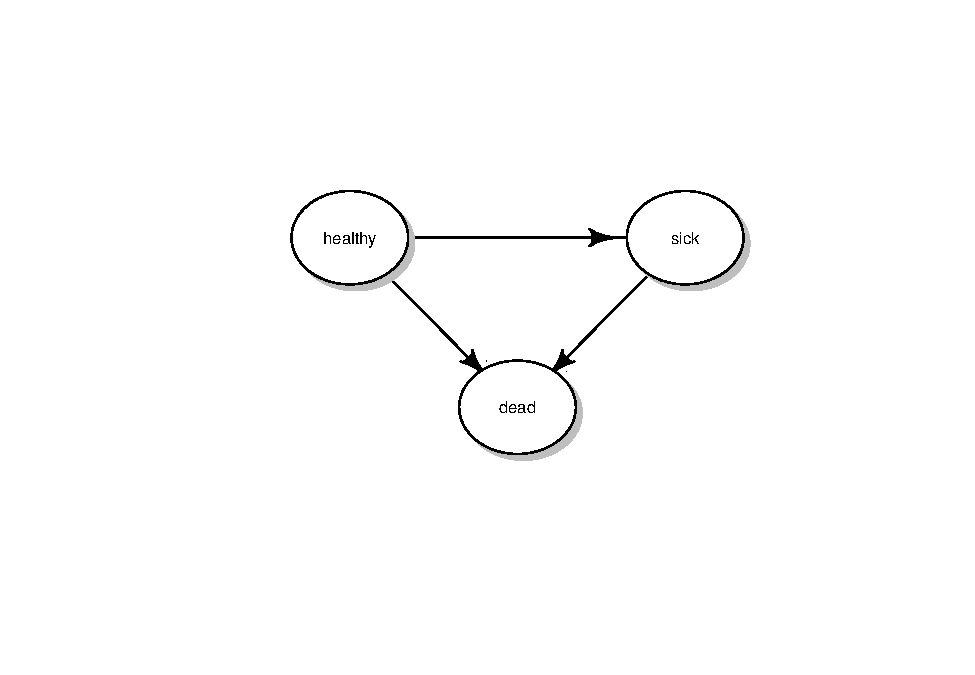
\includegraphics{Markov_3state_hesim_files/figure-latex/unnamed-chunk-5-1.pdf}

\hypertarget{define-and-initialize-matrices-and-vectors}{%
\section{04 Define and initialize matrices and
vectors}\label{define-and-initialize-matrices-and-vectors}}

\hypertarget{cohort-trace}{%
\subsection{04.1 Cohort trace}\label{cohort-trace}}

\begin{Shaded}
\begin{Highlighting}[]
\CommentTok{# create the cohort trace}
\NormalTok{m_M_SoC <-}\StringTok{ }\NormalTok{m_M_trt <-}\StringTok{  }\KeywordTok{matrix}\NormalTok{(}\OtherTok{NA}\NormalTok{, }
                              \DataTypeTok{nrow =}\NormalTok{ n_t }\OperatorTok{+}\StringTok{ }\DecValTok{1}\NormalTok{ ,  }\CommentTok{# create Markov trace (n_t + 1 because R doesn't }
                                                \CommentTok{# understand Cycle 0)}
                              \DataTypeTok{ncol =}\NormalTok{ n_states, }
                              \DataTypeTok{dimnames =} \KeywordTok{list}\NormalTok{(}\DecValTok{0}\OperatorTok{:}\NormalTok{n_t, v_n))}

\NormalTok{m_M_SoC[}\DecValTok{1}\NormalTok{, ] <-}\StringTok{ }\NormalTok{m_M_trt[}\DecValTok{1}\NormalTok{, ] <-}\StringTok{ }\NormalTok{v_init          }\CommentTok{# initialize first cycle of Markov trace}
\end{Highlighting}
\end{Shaded}

\hypertarget{transition-probability-matrix}{%
\subsection{04.2 Transition probability
matrix}\label{transition-probability-matrix}}

\begin{Shaded}
\begin{Highlighting}[]
\CommentTok{# create the transition probability matrices}
\NormalTok{m_P_SoC  <-}\StringTok{ }\NormalTok{m_P_trt <-}\StringTok{ }\KeywordTok{matrix}\NormalTok{(}\DecValTok{0}\NormalTok{,}
                              \DataTypeTok{nrow =}\NormalTok{ n_states, }\DataTypeTok{ncol =}\NormalTok{ n_states,}
                              \DataTypeTok{dimnames =} \KeywordTok{list}\NormalTok{(v_n, v_n))  }\CommentTok{# name the columns and rows of the matrix }
                                               
\CommentTok{# print the probability matrices }
\NormalTok{m_P_SoC  }\CommentTok{# for standard of care}
\end{Highlighting}
\end{Shaded}

\begin{verbatim}
##         Healthy Sick Dead
## Healthy       0    0    0
## Sick          0    0    0
## Dead          0    0    0
\end{verbatim}

\begin{Shaded}
\begin{Highlighting}[]
\NormalTok{m_P_trt  }\CommentTok{# treatment}
\end{Highlighting}
\end{Shaded}

\begin{verbatim}
##         Healthy Sick Dead
## Healthy       0    0    0
## Sick          0    0    0
## Dead          0    0    0
\end{verbatim}

Fill in the transition probability matrix:

\begin{Shaded}
\begin{Highlighting}[]
\CommentTok{# For Standard of Care }
\CommentTok{# from Healthy}
\NormalTok{m_P_SoC[}\StringTok{"Healthy"}\NormalTok{, }\StringTok{"Healthy"}\NormalTok{] <-}\StringTok{ }\NormalTok{(}\DecValTok{1} \OperatorTok{-}\StringTok{ }\NormalTok{p_HD) }\OperatorTok{*}\StringTok{ }\NormalTok{(}\DecValTok{1} \OperatorTok{-}\StringTok{ }\NormalTok{p_HS)}
\NormalTok{m_P_SoC[}\StringTok{"Healthy"}\NormalTok{, }\StringTok{"Sick"}\NormalTok{]    <-}\StringTok{ }\NormalTok{(}\DecValTok{1} \OperatorTok{-}\StringTok{ }\NormalTok{p_HD) }\OperatorTok{*}\StringTok{ }\NormalTok{p_HS}
\NormalTok{m_P_SoC[}\StringTok{"Healthy"}\NormalTok{, }\StringTok{"Dead"}\NormalTok{]    <-}\StringTok{ }\NormalTok{p_HD}

\CommentTok{# from Sick}
\NormalTok{m_P_SoC[}\StringTok{"Sick"}\NormalTok{, }\StringTok{"Sick"}\NormalTok{] <-}\StringTok{ }\DecValTok{1} \OperatorTok{-}\StringTok{ }\NormalTok{p_SD}
\NormalTok{m_P_SoC[}\StringTok{"Sick"}\NormalTok{, }\StringTok{"Dead"}\NormalTok{] <-}\StringTok{ }\NormalTok{p_SD}

\CommentTok{# from Dead}
\NormalTok{m_P_SoC[}\StringTok{"Dead"}\NormalTok{, }\StringTok{"Dead"}\NormalTok{] <-}\StringTok{ }\DecValTok{1}

\CommentTok{# Under treatment}
\NormalTok{m_P_trt <-}\StringTok{ }\NormalTok{m_P_SoC  }\CommentTok{# Assign the matrix for standard of care to the transition probability matrix for treatment}
\CommentTok{# replace values that are different under treatment }
\NormalTok{m_P_trt[}\StringTok{"Healthy"}\NormalTok{, }\StringTok{"Healthy"}\NormalTok{] <-}\StringTok{ }\NormalTok{(}\DecValTok{1} \OperatorTok{-}\StringTok{ }\NormalTok{p_HD) }\OperatorTok{*}\StringTok{ }\NormalTok{(}\DecValTok{1} \OperatorTok{-}\StringTok{ }\NormalTok{p_HS_trt)}
\NormalTok{m_P_trt[}\StringTok{"Healthy"}\NormalTok{, }\StringTok{"Sick"}\NormalTok{]    <-}\StringTok{ }\NormalTok{(}\DecValTok{1} \OperatorTok{-}\StringTok{ }\NormalTok{p_HD) }\OperatorTok{*}\StringTok{ }\NormalTok{p_HS_trt}
\end{Highlighting}
\end{Shaded}

\hypertarget{check-if-transition-probability-structure-and-probabilities-are-valid}{%
\subsection{04.3 Check if transition probability structure and
probabilities are
valid}\label{check-if-transition-probability-structure-and-probabilities-are-valid}}

\begin{Shaded}
\begin{Highlighting}[]
\CommentTok{# Check that transition probabilities are in [0, 1]}
\KeywordTok{check_transition_probability}\NormalTok{(m_P_SoC, }\DataTypeTok{verbose =} \OtherTok{TRUE}\NormalTok{)}
\KeywordTok{check_transition_probability}\NormalTok{(m_P_trt, }\DataTypeTok{verbose =} \OtherTok{TRUE}\NormalTok{)}
\CommentTok{# Check that all rows sum to 1}
\KeywordTok{check_sum_of_transition_array}\NormalTok{(m_P_SoC, }\DataTypeTok{n_states =}\NormalTok{ n_states, }\DataTypeTok{n_cycles =}\NormalTok{ n_t, }\DataTypeTok{verbose =} \OtherTok{TRUE}\NormalTok{)}
\KeywordTok{check_sum_of_transition_array}\NormalTok{(m_P_trt, }\DataTypeTok{n_states =}\NormalTok{ n_states, }\DataTypeTok{n_cycles =}\NormalTok{ n_t, }\DataTypeTok{verbose =} \OtherTok{TRUE}\NormalTok{)}
\end{Highlighting}
\end{Shaded}

\hypertarget{run-markov-model}{%
\section{05 Run Markov model}\label{run-markov-model}}

\begin{Shaded}
\begin{Highlighting}[]
\ControlFlowTok{for}\NormalTok{ (t }\ControlFlowTok{in} \DecValTok{1}\OperatorTok{:}\NormalTok{n_t)\{  }\CommentTok{# loop through the number of cycles}
\NormalTok{  m_M_SoC[t }\OperatorTok{+}\StringTok{ }\DecValTok{1}\NormalTok{, ] <-}\StringTok{ }\NormalTok{m_M_SoC[t, ] }\OperatorTok\StringTok{ }\NormalTok{m_P_SoC  }\CommentTok{# estimate the state vector for the next cycle (t + 1)}
\NormalTok{  m_M_trt[t }\OperatorTok{+}\StringTok{ }\DecValTok{1}\NormalTok{, ] <-}\StringTok{ }\NormalTok{m_M_trt[t, ] }\OperatorTok\StringTok{ }\NormalTok{m_P_trt  }\CommentTok{# for treatment}
\NormalTok{\}}
\end{Highlighting}
\end{Shaded}

\hypertarget{compute-and-plot-epidemiological-outcomes}{%
\section{06 Compute and Plot Epidemiological
Outcomes}\label{compute-and-plot-epidemiological-outcomes}}

\hypertarget{cohort-trace-1}{%
\subsection{06.1 Cohort trace}\label{cohort-trace-1}}

Standard of Care:

\begin{Shaded}
\begin{Highlighting}[]
\KeywordTok{matplot}\NormalTok{(m_M_SoC, }\DataTypeTok{type =} \StringTok{'l'}\NormalTok{, }
        \DataTypeTok{ylab =} \StringTok{"Probability of state occupancy"}\NormalTok{,}
        \DataTypeTok{xlab =} \StringTok{"Cycle"}\NormalTok{,}
        \DataTypeTok{main =} \StringTok{"Cohort Trace - standard of care"}\NormalTok{, }\DataTypeTok{lwd =} \DecValTok{3}\NormalTok{)  }\CommentTok{# create a plot of the data}
\KeywordTok{legend}\NormalTok{(}\StringTok{"right"}\NormalTok{, v_n, }\DataTypeTok{col =} \KeywordTok{c}\NormalTok{(}\StringTok{"black"}\NormalTok{, }\StringTok{"red"}\NormalTok{, }\StringTok{"green"}\NormalTok{), }
       \DataTypeTok{lty =} \DecValTok{1}\OperatorTok{:}\DecValTok{3}\NormalTok{, }\DataTypeTok{bty =} \StringTok{"n"}\NormalTok{)                            }\CommentTok{# add a legend to the graph}

\KeywordTok{abline}\NormalTok{(}\DataTypeTok{v =} \KeywordTok{which.max}\NormalTok{(m_M_SoC[, }\StringTok{"Sick"}\NormalTok{]), }\DataTypeTok{col =} \StringTok{"gray"}\NormalTok{)      }\CommentTok{# plot a vertical line that helps identifying at which cycle the prevalence of sick is highest.  }
\end{Highlighting}
\end{Shaded}

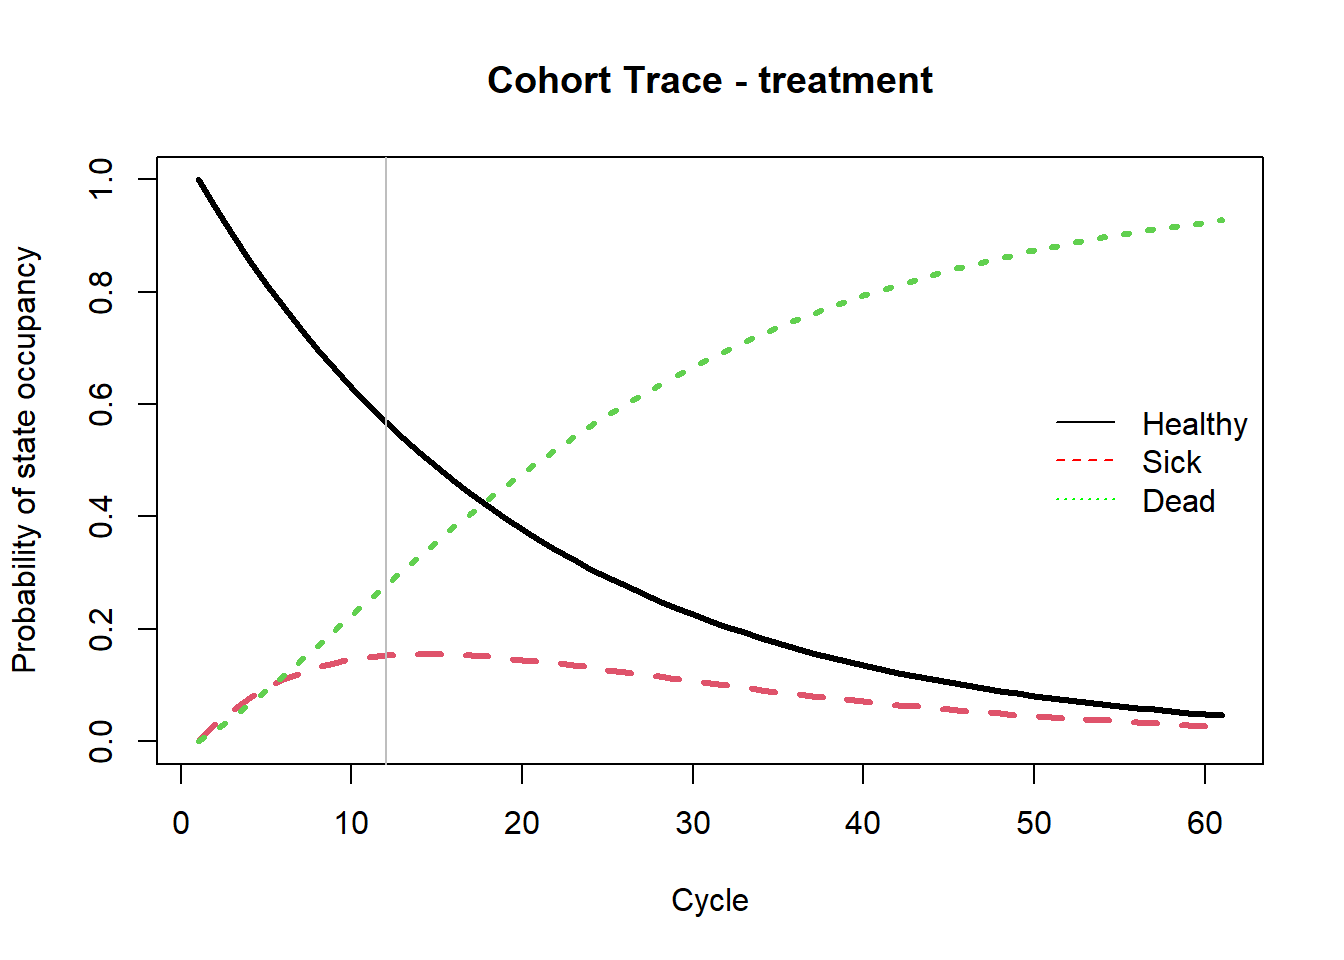
\includegraphics{Markov_3state_hesim_files/figure-latex/unnamed-chunk-11-1.pdf}

Treatment:

\begin{Shaded}
\begin{Highlighting}[]
\KeywordTok{matplot}\NormalTok{(m_M_trt, }\DataTypeTok{type =} \StringTok{'l'}\NormalTok{, }
        \DataTypeTok{ylab =} \StringTok{"Probability of state occupancy"}\NormalTok{,}
        \DataTypeTok{xlab =} \StringTok{"Cycle"}\NormalTok{,}
        \DataTypeTok{main =} \StringTok{"Cohort Trace - treatment"}\NormalTok{, }\DataTypeTok{lwd =} \DecValTok{3}\NormalTok{)     }\CommentTok{# create a plot of the data}
\KeywordTok{legend}\NormalTok{(}\StringTok{"right"}\NormalTok{, v_n, }\DataTypeTok{col =} \KeywordTok{c}\NormalTok{(}\StringTok{"black"}\NormalTok{, }\StringTok{"red"}\NormalTok{, }\StringTok{"green"}\NormalTok{), }
       \DataTypeTok{lty =} \DecValTok{1}\OperatorTok{:}\DecValTok{3}\NormalTok{, }\DataTypeTok{bty =} \StringTok{"n"}\NormalTok{)                            }\CommentTok{# add a legend to the graph}

\KeywordTok{abline}\NormalTok{(}\DataTypeTok{v =} \KeywordTok{which.max}\NormalTok{(m_M_trt[, }\StringTok{"Sick"}\NormalTok{]), }\DataTypeTok{col =} \StringTok{"gray"}\NormalTok{)      }\CommentTok{# plot a vertical line that helps identifying at which cycle the prevalence of sick is highest.  }
\end{Highlighting}
\end{Shaded}

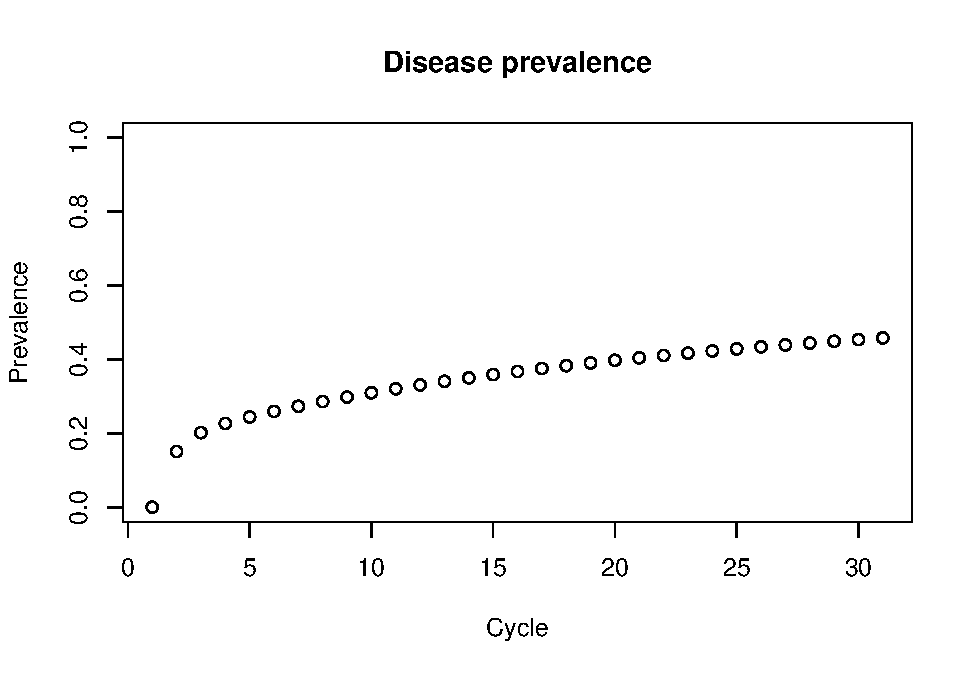
\includegraphics{Markov_3state_hesim_files/figure-latex/unnamed-chunk-12-1.pdf}

\hypertarget{overall-survival-os}{%
\subsection{06.2 Overall Survival (OS)}\label{overall-survival-os}}

Standard of Care:

\begin{Shaded}
\begin{Highlighting}[]
\NormalTok{v_os_SoC <-}\StringTok{ }\DecValTok{1} \OperatorTok{-}\StringTok{ }\NormalTok{m_M_SoC[, }\StringTok{"Dead"}\NormalTok{]    }\CommentTok{# calculate the overall survival (OS) probability}
\NormalTok{v_os_SoC <-}\StringTok{ }\KeywordTok{rowSums}\NormalTok{(m_M_SoC[, }\DecValTok{1}\OperatorTok{:}\DecValTok{2}\NormalTok{])  }\CommentTok{# alternative way of calculating the OS probability   }

\KeywordTok{plot}\NormalTok{(v_os_SoC, }\DataTypeTok{type =} \StringTok{'l'}\NormalTok{, }
     \DataTypeTok{ylim =} \KeywordTok{c}\NormalTok{(}\DecValTok{0}\NormalTok{, }\DecValTok{1}\NormalTok{),}
     \DataTypeTok{ylab =} \StringTok{"Survival probability"}\NormalTok{,}
     \DataTypeTok{xlab =} \StringTok{"Cycle"}\NormalTok{,}
     \DataTypeTok{main =} \StringTok{"Overall Survival - Standard of Care"}\NormalTok{)  }\CommentTok{# create a simple plot showing the OS}

\CommentTok{# add grid }
\KeywordTok{grid}\NormalTok{(}\DataTypeTok{nx =}\NormalTok{ n_t, }\DataTypeTok{ny =} \DecValTok{10}\NormalTok{, }\DataTypeTok{col =} \StringTok{"lightgray"}\NormalTok{, }\DataTypeTok{lty =} \StringTok{"dotted"}\NormalTok{, }\DataTypeTok{lwd =} \KeywordTok{par}\NormalTok{(}\StringTok{"lwd"}\NormalTok{), }
     \DataTypeTok{equilogs =} \OtherTok{TRUE}\NormalTok{) }
\end{Highlighting}
\end{Shaded}

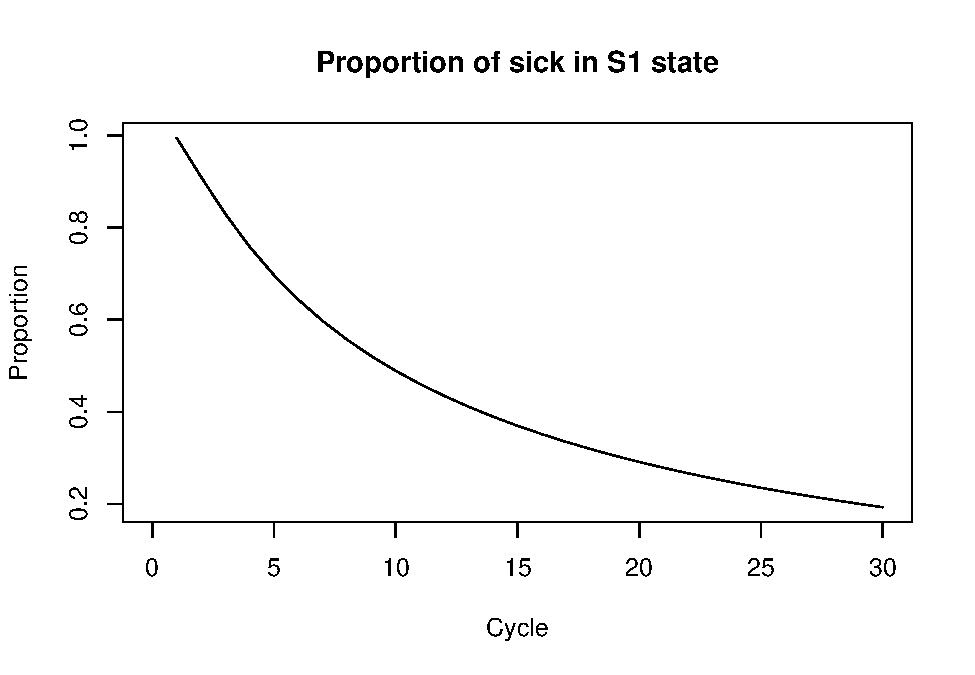
\includegraphics{Markov_3state_hesim_files/figure-latex/unnamed-chunk-13-1.pdf}

Treatment:

\begin{Shaded}
\begin{Highlighting}[]
\NormalTok{v_os_trt <-}\StringTok{ }\DecValTok{1} \OperatorTok{-}\StringTok{ }\NormalTok{m_M_trt[, }\StringTok{"Dead"}\NormalTok{]    }\CommentTok{# calculate the overall survival (OS) probability}
\NormalTok{v_os_trt <-}\StringTok{ }\KeywordTok{rowSums}\NormalTok{(m_M_trt[, }\DecValTok{1}\OperatorTok{:}\DecValTok{2}\NormalTok{])  }\CommentTok{# alternative way of calculating the OS probability}

\KeywordTok{plot}\NormalTok{(v_os_trt, }\DataTypeTok{type =} \StringTok{'l'}\NormalTok{, }
     \DataTypeTok{ylim =} \KeywordTok{c}\NormalTok{(}\DecValTok{0}\NormalTok{, }\DecValTok{1}\NormalTok{),}
     \DataTypeTok{ylab =} \StringTok{"Survival probability"}\NormalTok{,}
     \DataTypeTok{xlab =} \StringTok{"Cycle"}\NormalTok{,}
     \DataTypeTok{main =} \StringTok{"Overall Survival - Treatment"}\NormalTok{)  }\CommentTok{# create a simple plot showing the OS}

\CommentTok{# add grid }
\KeywordTok{grid}\NormalTok{(}\DataTypeTok{nx =}\NormalTok{ n_t, }\DataTypeTok{ny =} \DecValTok{10}\NormalTok{, }\DataTypeTok{col =} \StringTok{"lightgray"}\NormalTok{, }\DataTypeTok{lty =} \StringTok{"dotted"}\NormalTok{, }\DataTypeTok{lwd =} \KeywordTok{par}\NormalTok{(}\StringTok{"lwd"}\NormalTok{), }
     \DataTypeTok{equilogs =} \OtherTok{TRUE}\NormalTok{) }
\end{Highlighting}
\end{Shaded}

\includegraphics{Markov_3state_hesim_files/figure-latex/unnamed-chunk-14-1.pdf}

\hypertarget{life-expectancy-le}{%
\subsection{06.2.1 Life Expectancy (LE)}\label{life-expectancy-le}}

\begin{Shaded}
\begin{Highlighting}[]
\NormalTok{v_le_SoC <-}\StringTok{ }\KeywordTok{sum}\NormalTok{(v_os_SoC)  }\CommentTok{# summing probability of OS over time (i.e. life expectancy)}
\NormalTok{v_le_trt <-}\StringTok{ }\KeywordTok{sum}\NormalTok{(v_os_trt)  }\CommentTok{# summing probability of OS over time (i.e. life expectancy), treatment}
\end{Highlighting}
\end{Shaded}

\hypertarget{disease-prevalence}{%
\subsection{06.3 Disease prevalence}\label{disease-prevalence}}

Standard of Care:

\begin{Shaded}
\begin{Highlighting}[]
\NormalTok{v_prev_SoC <-}\StringTok{ }\NormalTok{m_M_SoC[, }\StringTok{"Sick"}\NormalTok{]}\OperatorTok{/}\NormalTok{v_os_SoC}
\KeywordTok{plot}\NormalTok{(v_prev_SoC,}
     \DataTypeTok{ylim =} \KeywordTok{c}\NormalTok{(}\DecValTok{0}\NormalTok{, }\DecValTok{1}\NormalTok{),}
     \DataTypeTok{ylab =} \StringTok{"Prevalence"}\NormalTok{,}
     \DataTypeTok{xlab =} \StringTok{"Cycle"}\NormalTok{,}
     \DataTypeTok{main =} \StringTok{"Disease prevalence - Standard of care"}\NormalTok{)}
\end{Highlighting}
\end{Shaded}

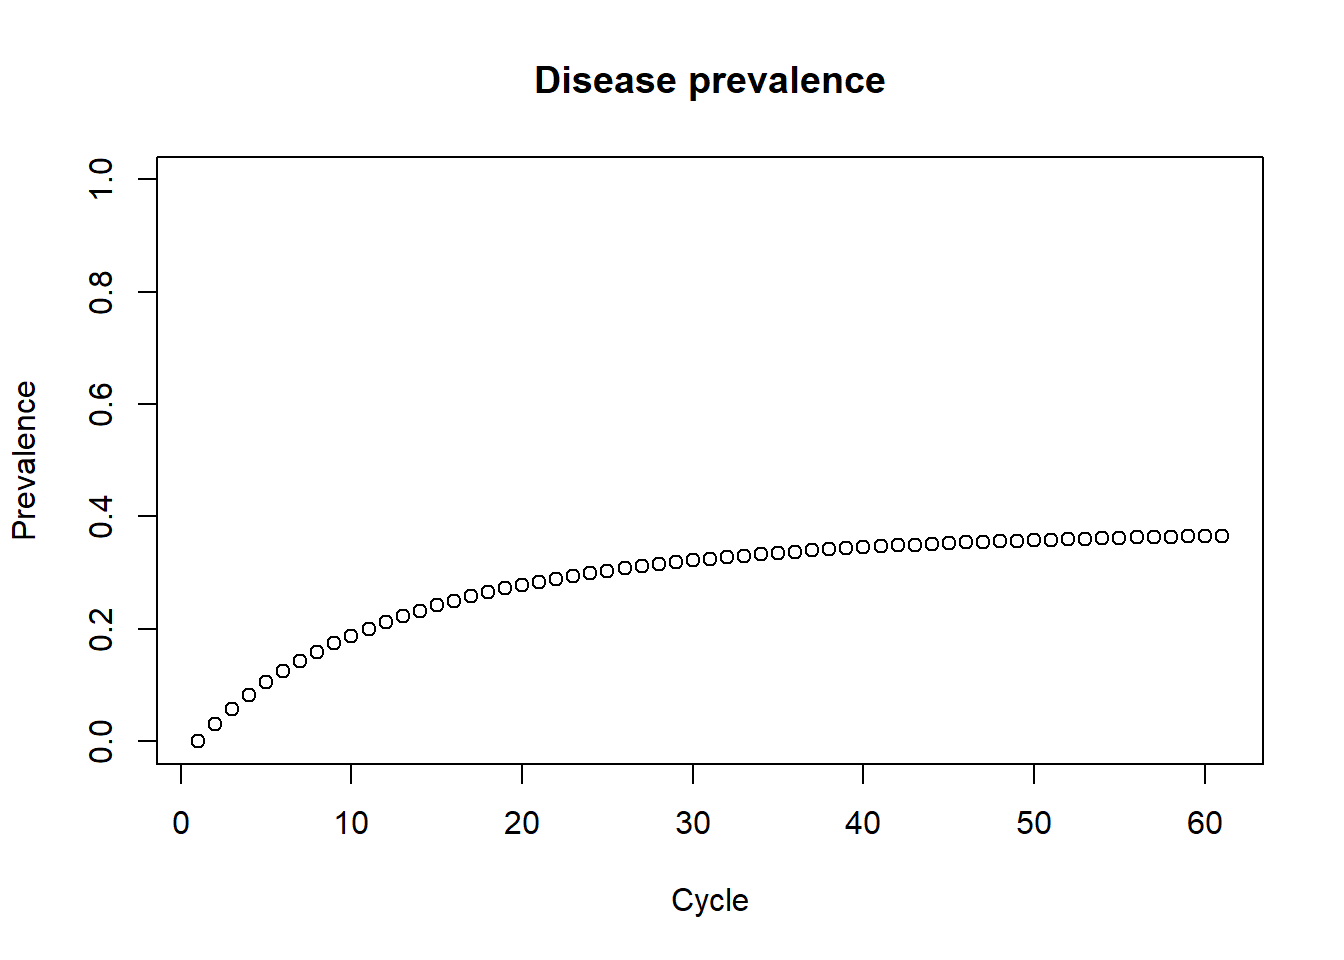
\includegraphics{Markov_3state_hesim_files/figure-latex/unnamed-chunk-16-1.pdf}

Treatment:

\begin{Shaded}
\begin{Highlighting}[]
\NormalTok{v_prev_trt <-}\StringTok{ }\NormalTok{m_M_trt[, }\StringTok{"Sick"}\NormalTok{]}\OperatorTok{/}\NormalTok{v_os_trt}
\KeywordTok{plot}\NormalTok{(v_prev_trt,}
     \DataTypeTok{ylim =} \KeywordTok{c}\NormalTok{(}\DecValTok{0}\NormalTok{, }\DecValTok{1}\NormalTok{),}
     \DataTypeTok{ylab =} \StringTok{"Prevalence"}\NormalTok{,}
     \DataTypeTok{xlab =} \StringTok{"Cycle"}\NormalTok{,}
     \DataTypeTok{main =} \StringTok{"Disease prevalence - Treatment"}\NormalTok{)}
\end{Highlighting}
\end{Shaded}

\includegraphics{Markov_3state_hesim_files/figure-latex/unnamed-chunk-17-1.pdf}

\hypertarget{compute-cost-effectiveness-outcomes}{%
\section{07 Compute Cost-Effectiveness
Outcomes}\label{compute-cost-effectiveness-outcomes}}

\hypertarget{mean-costs-and-qalys}{%
\subsection{07.1 Mean Costs and QALYs}\label{mean-costs-and-qalys}}

\begin{Shaded}
\begin{Highlighting}[]
\CommentTok{# per cycle}
\CommentTok{# calculate expected costs by multiplying m_M with the cost vector for the different }
\CommentTok{# health states   }
\NormalTok{v_tc_SoC <-}\StringTok{ }\NormalTok{m_M_SoC }\OperatorTok\StringTok{ }\KeywordTok{c}\NormalTok{(c_H, c_S, c_D)  }\CommentTok{# Standard of Care}
\NormalTok{v_tc_trt <-}\StringTok{ }\NormalTok{m_M_trt }\OperatorTok\StringTok{ }\KeywordTok{c}\NormalTok{(c_H, c_S, c_D)  }\CommentTok{# Treatment}
\NormalTok{v_tc_trt[}\DecValTok{1}\NormalTok{] <-}\StringTok{ }\NormalTok{v_tc_trt[}\DecValTok{1}\NormalTok{] }\OperatorTok{+}\StringTok{ }\NormalTok{c_trt}
\CommentTok{# calculate expected QALYs by multiplying m_M with the utilities for the different }
\CommentTok{# health states   }
\NormalTok{v_tu_SoC <-}\StringTok{ }\NormalTok{m_M_SoC }\OperatorTok\StringTok{ }\KeywordTok{c}\NormalTok{(u_H, u_S, u_D)  }\CommentTok{# Standard of Care}
\NormalTok{v_tu_trt <-}\StringTok{ }\NormalTok{m_M_trt }\OperatorTok\StringTok{ }\KeywordTok{c}\NormalTok{(u_H, u_S, u_D)  }\CommentTok{# Treatment}
\end{Highlighting}
\end{Shaded}

\hypertarget{discounted-mean-costs-and-qalys}{%
\subsection{07.2 Discounted Mean Costs and
QALYs}\label{discounted-mean-costs-and-qalys}}

\begin{Shaded}
\begin{Highlighting}[]
\CommentTok{# Discount costs by multiplying the cost vector with discount weights  }
\NormalTok{tc_d_SoC  <-}\StringTok{  }\KeywordTok{t}\NormalTok{(v_tc_SoC) }\OperatorTok\StringTok{ }\NormalTok{v_dwc  }\CommentTok{# Standard of Care}
\NormalTok{tc_d_trt  <-}\StringTok{  }\KeywordTok{t}\NormalTok{(v_tc_trt) }\OperatorTok\StringTok{ }\NormalTok{v_dwc  }\CommentTok{# Treatment}
\CommentTok{# Discount QALYS by multiplying the QALYs vector with discount weights }
\NormalTok{tu_d_SoC  <-}\StringTok{  }\KeywordTok{t}\NormalTok{(v_tu_SoC) }\OperatorTok\StringTok{ }\NormalTok{v_dwe  }\CommentTok{# Standard of Care}
\NormalTok{tu_d_trt  <-}\StringTok{  }\KeywordTok{t}\NormalTok{(v_tu_trt) }\OperatorTok\StringTok{ }\NormalTok{v_dwe  }\CommentTok{# Treatment}

\CommentTok{# store them into a vector}
\NormalTok{v_tc_d    <-}\StringTok{ }\KeywordTok{c}\NormalTok{(tc_d_SoC, tc_d_trt)}
\NormalTok{v_tu_d    <-}\StringTok{ }\KeywordTok{c}\NormalTok{(tu_d_SoC, tu_d_trt)}

\CommentTok{# Dataframe with discounted costs and effectiveness}
\NormalTok{df_ce       <-}\StringTok{ }\KeywordTok{data.frame}\NormalTok{(}\DataTypeTok{Strategy =}\NormalTok{ v_names_str,}
                          \DataTypeTok{Cost     =}\NormalTok{ v_tc_d,}
                          \DataTypeTok{Effect   =}\NormalTok{ v_tu_d)}
\NormalTok{df_ce}
\end{Highlighting}
\end{Shaded}

\begin{verbatim}
##           Strategy      Cost   Effect
## 1 Standard of Care  8043.139 10.25087
## 2        Treatment 16028.490 11.73928
\end{verbatim}

\hypertarget{compute-icers-of-the-markov-model}{%
\subsection{07.3 Compute ICERs of the Markov
model}\label{compute-icers-of-the-markov-model}}

\begin{Shaded}
\begin{Highlighting}[]
\NormalTok{df_cea <-}\StringTok{ }\KeywordTok{calculate_icers}\NormalTok{(}\DataTypeTok{cost       =}\NormalTok{ df_ce}\OperatorTok{$}\NormalTok{Cost,}
                          \DataTypeTok{effect     =}\NormalTok{ df_ce}\OperatorTok{$}\NormalTok{Effect,}
                          \DataTypeTok{strategies =}\NormalTok{ df_ce}\OperatorTok{$}\NormalTok{Strategy)}
\NormalTok{df_cea}
\end{Highlighting}
\end{Shaded}

\begin{verbatim}
##           Strategy      Cost   Effect Inc_Cost Inc_Effect     ICER Status
## 1 Standard of Care  8043.139 10.25087       NA         NA       NA     ND
## 2        Treatment 16028.490 11.73928 7985.351   1.488415 5365.002     ND
\end{verbatim}

\hypertarget{plot-frontier-of-the-markov-model}{%
\subsection{07.4 Plot frontier of the Markov
model}\label{plot-frontier-of-the-markov-model}}

\begin{Shaded}
\begin{Highlighting}[]
\KeywordTok{plot}\NormalTok{(df_cea, }\DataTypeTok{effect_units =} \StringTok{"QALYs"}\NormalTok{, }\DataTypeTok{xlim =} \KeywordTok{c}\NormalTok{(}\DecValTok{10}\NormalTok{, }\DecValTok{12}\NormalTok{))}
\end{Highlighting}
\end{Shaded}

\includegraphics{Markov_3state_hesim_files/figure-latex/unnamed-chunk-21-1.pdf}

\begin{Shaded}
\begin{Highlighting}[]
\CommentTok{# note: you need to adjust the xlim values to values that are covering the range of effect values in your analysis}
\end{Highlighting}
\end{Shaded}

\hypertarget{probabilistic-sensitivity-analysis-psa}{%
\section{08 Probabilistic Sensitivity Analysis
(PSA)}\label{probabilistic-sensitivity-analysis-psa}}

\hypertarget{list-of-input-parameters}{%
\subsection{08.1 List of input
parameters}\label{list-of-input-parameters}}

Create list \texttt{l\_params\_all} with all input probabilities, cost
and utilities.

\begin{Shaded}
\begin{Highlighting}[]
\NormalTok{l_params_all <-}\StringTok{ }\KeywordTok{as.list}\NormalTok{(}\KeywordTok{data.frame}\NormalTok{(}
  \DataTypeTok{p_HD     =} \FloatTok{0.02}\NormalTok{,  }\CommentTok{# probability of dying when healthy}
  \DataTypeTok{p_HS     =} \FloatTok{0.05}\NormalTok{,  }\CommentTok{# probability of becoming sick when healthy, conditioned on not dying}
  \DataTypeTok{p_HS_trt =} \FloatTok{0.03}\NormalTok{,  }\CommentTok{# probability of becoming sick when healthy, conditioned on not dying}
  \DataTypeTok{p_SD     =} \FloatTok{0.1}\NormalTok{,   }\CommentTok{# probability of dying when sick}
  \DataTypeTok{c_H      =} \DecValTok{400}\NormalTok{,   }\CommentTok{# cost of one cycle in healthy state}
  \DataTypeTok{c_S      =} \DecValTok{1000}\NormalTok{,  }\CommentTok{# cost of one cycle in sick state}
  \DataTypeTok{c_D      =} \DecValTok{0}\NormalTok{,     }\CommentTok{# cost of one cycle in dead state}
  \DataTypeTok{c_trt    =} \DecValTok{8000}\NormalTok{,   }\CommentTok{# one-time cost of treatment (at first cycle)}
  \DataTypeTok{u_H      =} \FloatTok{0.8}\NormalTok{,   }\CommentTok{# utility when healthy }
  \DataTypeTok{u_S      =} \FloatTok{0.5}\NormalTok{,   }\CommentTok{# utility when sick}
  \DataTypeTok{u_D      =} \DecValTok{0}\NormalTok{,     }\CommentTok{# utility when dead}
  \DataTypeTok{d_e      =} \FloatTok{0.03}\NormalTok{,  }\CommentTok{# discount factor for effectiveness}
  \DataTypeTok{d_c      =} \FloatTok{0.03}   \CommentTok{# discount factor for costs}
\NormalTok{))}

\CommentTok{# store the parameter names into a vector}
\NormalTok{v_names_params <-}\StringTok{ }\KeywordTok{names}\NormalTok{(l_params_all)}
\end{Highlighting}
\end{Shaded}

\hypertarget{load-sick-sicker-markov-model-function}{%
\subsection{08.2 Load Sick-Sicker Markov model
function}\label{load-sick-sicker-markov-model-function}}

\begin{Shaded}
\begin{Highlighting}[]
\KeywordTok{source}\NormalTok{(}\StringTok{"Functions_markov_3state.R"}\NormalTok{)}
\CommentTok{# Test function}
\KeywordTok{calculate_ce_out}\NormalTok{(l_params_all)}
\end{Highlighting}
\end{Shaded}

\begin{verbatim}
##           Strategy      Cost   Effect       NMB
## 1 Standard of Care  8043.139 10.25087  94465.51
## 2        Treatment 16028.490 11.73928 101364.32
\end{verbatim}

\hypertarget{generate-psa-datasets}{%
\subsection{08.3 Generate PSA datasets}\label{generate-psa-datasets}}

\begin{Shaded}
\begin{Highlighting}[]
\CommentTok{# Function to generate PSA input dataset}
\NormalTok{gen_psa <-}\StringTok{ }\ControlFlowTok{function}\NormalTok{(}\DataTypeTok{n_sim =} \DecValTok{1000}\NormalTok{, }\DataTypeTok{seed =} \DecValTok{071818}\NormalTok{)\{}
  \KeywordTok{set.seed}\NormalTok{(seed) }\CommentTok{# set a seed to be able to reproduce the same results}
\NormalTok{  df_psa <-}\StringTok{ }\KeywordTok{data.frame}\NormalTok{(}
    \CommentTok{# Transition probabilities (per cycle)}
    \CommentTok{# probability to become sick when healthy}
    \DataTypeTok{p_HS     =} \KeywordTok{rbeta}\NormalTok{(n_sim, }\DataTypeTok{shape1 =} \DecValTok{24}\NormalTok{, }\DataTypeTok{shape2 =} \DecValTok{450}\NormalTok{), }
    \DataTypeTok{p_HS_trt =} \KeywordTok{rbeta}\NormalTok{(n_sim, }\DataTypeTok{shape1 =} \DecValTok{9}\NormalTok{,  }\DataTypeTok{shape2 =} \DecValTok{281}\NormalTok{),   }\CommentTok{# under treatment}
    \CommentTok{# probability of dying when healthy}
    \DataTypeTok{p_HD     =} \KeywordTok{rbeta}\NormalTok{(n_sim, }\DataTypeTok{shape1 =} \DecValTok{16}\NormalTok{, }\DataTypeTok{shape2 =} \DecValTok{767}\NormalTok{),}
    \CommentTok{# probability of dying when sick}
    \DataTypeTok{p_SD     =} \KeywordTok{rbeta}\NormalTok{(n_sim, }\DataTypeTok{shape1 =} \FloatTok{22.4}\NormalTok{, }\DataTypeTok{shape2 =} \FloatTok{201.6}\NormalTok{), }

    \CommentTok{# Cost vectors with length n_sim}
    \CommentTok{# cost of remaining one cycle in state H}
    \DataTypeTok{c_H      =} \KeywordTok{rgamma}\NormalTok{(n_sim, }\DataTypeTok{shape =} \DecValTok{16}\NormalTok{, }\DataTypeTok{scale =} \DecValTok{25}\NormalTok{), }
    \CommentTok{# cost of remaining one cycle in state S1}
    \DataTypeTok{c_S      =} \KeywordTok{rgamma}\NormalTok{(n_sim, }\DataTypeTok{shape =} \DecValTok{100}\NormalTok{, }\DataTypeTok{scale =} \DecValTok{10}\NormalTok{), }
    \CommentTok{# cost of being in the death state}
    \DataTypeTok{c_D      =} \DecValTok{0}\NormalTok{, }
    \CommentTok{# cost of treatment (per cycle)}
    \DataTypeTok{c_trt    =} \KeywordTok{rgamma}\NormalTok{(n_sim, }\DataTypeTok{shape =} \DecValTok{64}\NormalTok{, }\DataTypeTok{scale =} \DecValTok{125}\NormalTok{),}
    
    \CommentTok{# Utility vectors with length n_sim }
    \CommentTok{# utility when healthy}
    \DataTypeTok{u_H      =} \KeywordTok{rbeta}\NormalTok{(n_sim, }\DataTypeTok{shape1 =}  \FloatTok{50.4}\NormalTok{, }\DataTypeTok{shape2 =} \FloatTok{12.6}\NormalTok{), }
    \CommentTok{# utility when sick}
    \DataTypeTok{u_S      =} \KeywordTok{rbeta}\NormalTok{(n_sim, }\DataTypeTok{shape1 =} \FloatTok{49.5}\NormalTok{, }\DataTypeTok{shape2 =} \FloatTok{49.5}\NormalTok{), }
    \CommentTok{# utility when dead}
    \DataTypeTok{u_D      =} \DecValTok{0}                                              
\NormalTok{  )}
  \KeywordTok{return}\NormalTok{(df_psa)}
\NormalTok{\}}
\CommentTok{# Try it}
\KeywordTok{gen_psa}\NormalTok{(}\DecValTok{10}\NormalTok{) }
\end{Highlighting}
\end{Shaded}

\begin{verbatim}
##          p_HS   p_HS_trt       p_HD       p_SD      c_H       c_S c_D    c_trt
## 1  0.05116365 0.02717469 0.02650780 0.09350365 331.7253 1001.3478   0 6217.035
## 2  0.04095451 0.01181545 0.02787410 0.15823599 535.2239  995.9279   0 9377.706
## 3  0.05334926 0.01972404 0.01561002 0.12357583 334.2034  955.0140   0 6591.331
## 4  0.03627100 0.03901602 0.02620191 0.08771020 352.7561  990.4764   0 8652.337
## 5  0.04782122 0.02128019 0.01998096 0.10799984 260.4642  943.7245   0 8555.065
## 6  0.07206924 0.02272066 0.01521342 0.12685251 291.1215  983.1453   0 8604.577
## 7  0.04803791 0.04457119 0.01499307 0.08911761 483.8274 1050.5295   0 9942.503
## 8  0.04335723 0.02882206 0.02131098 0.05814786 541.4731  864.3322   0 6018.085
## 9  0.05302297 0.03409499 0.01709267 0.15922549 551.1535 1080.4473   0 7571.225
## 10 0.03096171 0.01553948 0.01983932 0.10406523 315.7027  984.6521   0 7875.281
##          u_H       u_S u_D
## 1  0.8559721 0.4815761   0
## 2  0.7783084 0.5349337   0
## 3  0.8628224 0.5227023   0
## 4  0.8968823 0.4871518   0
## 5  0.8179546 0.5294793   0
## 6  0.6717953 0.5249675   0
## 7  0.8177386 0.5600215   0
## 8  0.8145828 0.5243320   0
## 9  0.8153981 0.5503887   0
## 10 0.8835447 0.5837644   0
\end{verbatim}

\begin{Shaded}
\begin{Highlighting}[]
\CommentTok{# Number of simulations}
\NormalTok{n_sim <-}\StringTok{ }\DecValTok{1000}

\CommentTok{# Generate PSA input dataset}
\NormalTok{df_psa_input <-}\StringTok{ }\KeywordTok{gen_psa}\NormalTok{(}\DataTypeTok{n_sim =}\NormalTok{ n_sim)}
\CommentTok{# First six observations}
\KeywordTok{head}\NormalTok{(df_psa_input)}
\end{Highlighting}
\end{Shaded}

\begin{verbatim}
##         p_HS   p_HS_trt       p_HD       p_SD      c_H       c_S c_D     c_trt
## 1 0.05116365 0.01954245 0.02621456 0.13853135 307.8380  899.5153   0  6875.154
## 2 0.04095451 0.04346716 0.01760834 0.13075427 466.9600 1066.1617   0  8755.292
## 3 0.05334926 0.03357981 0.02404573 0.08454761 235.2890  955.0145   0  6582.810
## 4 0.03627100 0.03806155 0.02716409 0.10457346 306.5100  789.6969   0  7027.446
## 5 0.04782122 0.03737024 0.01716697 0.14474739 535.1188  868.0570   0  5661.605
## 6 0.07206924 0.04257367 0.01710648 0.12289879 353.6715  991.6205   0 10960.742
##         u_H       u_S u_D
## 1 0.7965014 0.4473598   0
## 2 0.7659582 0.4644020   0
## 3 0.7593770 0.4215045   0
## 4 0.8338376 0.5052819   0
## 5 0.8798517 0.5181703   0
## 6 0.7306958 0.5905503   0
\end{verbatim}

\begin{Shaded}
\begin{Highlighting}[]
\CommentTok{# Histogram of parameters}
\KeywordTok{ggplot}\NormalTok{(}\KeywordTok{melt}\NormalTok{(df_psa_input, }\DataTypeTok{variable.name =} \StringTok{"Parameter"}\NormalTok{), }\KeywordTok{aes}\NormalTok{(}\DataTypeTok{x =}\NormalTok{ value)) }\OperatorTok{+}
\StringTok{       }\KeywordTok{facet_wrap}\NormalTok{(}\OperatorTok{~}\NormalTok{Parameter, }\DataTypeTok{scales =} \StringTok{"free"}\NormalTok{) }\OperatorTok{+}
\StringTok{       }\KeywordTok{geom_histogram}\NormalTok{(}\KeywordTok{aes}\NormalTok{(}\DataTypeTok{y =}\NormalTok{ ..density..)) }\OperatorTok{+}
\StringTok{       }\KeywordTok{theme_bw}\NormalTok{(}\DataTypeTok{base_size =} \DecValTok{16}\NormalTok{) }\OperatorTok{+}\StringTok{ }
\StringTok{       }\KeywordTok{theme}\NormalTok{(}\DataTypeTok{axis.text =} \KeywordTok{element_text}\NormalTok{(}\DataTypeTok{size=}\DecValTok{8}\NormalTok{))}
\end{Highlighting}
\end{Shaded}

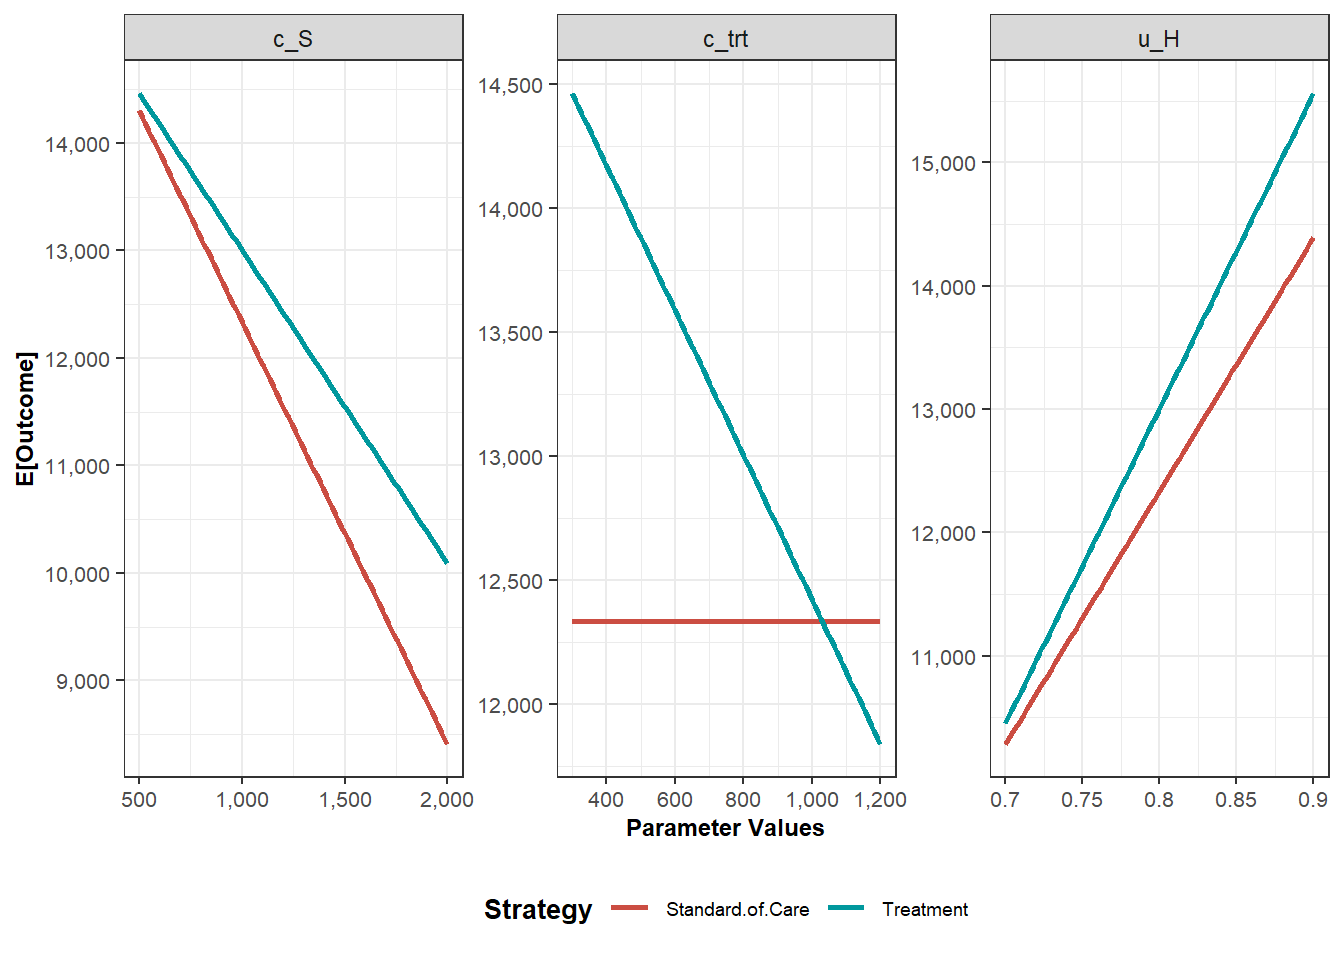
\includegraphics{Markov_3state_hesim_files/figure-latex/unnamed-chunk-24-1.pdf}

\begin{Shaded}
\begin{Highlighting}[]
\CommentTok{# Initialize dataframes with PSA output }
\CommentTok{# Dataframe of costs}
\NormalTok{df_c <-}\StringTok{ }\KeywordTok{as.data.frame}\NormalTok{(}\KeywordTok{matrix}\NormalTok{(}\DecValTok{0}\NormalTok{, }
                      \DataTypeTok{nrow =}\NormalTok{ n_sim,}
                      \DataTypeTok{ncol =}\NormalTok{ n_str))}
\KeywordTok{colnames}\NormalTok{(df_c) <-}\StringTok{ }\NormalTok{v_names_str}
\CommentTok{# Dataframe of effectiveness}
\NormalTok{df_e <-}\StringTok{ }\KeywordTok{as.data.frame}\NormalTok{(}\KeywordTok{matrix}\NormalTok{(}\DecValTok{0}\NormalTok{, }
                      \DataTypeTok{nrow =}\NormalTok{ n_sim,}
                      \DataTypeTok{ncol =}\NormalTok{ n_str))}
\KeywordTok{colnames}\NormalTok{(df_e) <-}\StringTok{ }\NormalTok{v_names_str}
\end{Highlighting}
\end{Shaded}

\hypertarget{conduct-probabilistic-sensitivity-analysis}{%
\subsection{08.4 Conduct probabilistic sensitivity
analysis}\label{conduct-probabilistic-sensitivity-analysis}}

\begin{Shaded}
\begin{Highlighting}[]
\CommentTok{# Run Markov model on each parameter set of PSA input dataset}
\ControlFlowTok{for}\NormalTok{(i }\ControlFlowTok{in} \DecValTok{1}\OperatorTok{:}\NormalTok{n_sim)\{}
\NormalTok{  l_out_temp <-}\StringTok{ }\KeywordTok{calculate_ce_out}\NormalTok{(df_psa_input[i, ])}
\NormalTok{  df_c[i, ] <-}\StringTok{ }\NormalTok{l_out_temp}\OperatorTok{$}\NormalTok{Cost}
\NormalTok{  df_e[i, ] <-}\StringTok{ }\NormalTok{l_out_temp}\OperatorTok{$}\NormalTok{Effect}
  \CommentTok{# Display simulation progress}
  \ControlFlowTok{if}\NormalTok{(i}\OperatorTok{/}\NormalTok{(n_sim}\OperatorTok{/}\DecValTok{10}\NormalTok{) }\OperatorTok{==}\StringTok{ }\KeywordTok{round}\NormalTok{(i}\OperatorTok{/}\NormalTok{(n_sim}\OperatorTok{/}\DecValTok{10}\NormalTok{), }\DecValTok{0}\NormalTok{)) \{ }\CommentTok{# display progress every 10%}
    \KeywordTok{cat}\NormalTok{(}\StringTok{'}\CharTok{\textbackslash{}r}\StringTok{'}\NormalTok{, }\KeywordTok{paste}\NormalTok{(i}\OperatorTok{/}\NormalTok{n_sim }\OperatorTok{*}\StringTok{ }\DecValTok{100}\NormalTok{, }\StringTok{"% done"}\NormalTok{, }\DataTypeTok{sep =} \StringTok{" "}\NormalTok{))}
\NormalTok{  \}}
\NormalTok{\}}
\end{Highlighting}
\end{Shaded}

\begin{verbatim}
##  10 % done 20 % done 30 % done 40 % done 50 % done 60 % done 70 % done 80 % done 90 % done 100 % done
\end{verbatim}

\hypertarget{create-psa-object-for-dampack}{%
\subsection{08.4.1 Create PSA object for
dampack}\label{create-psa-object-for-dampack}}

\begin{Shaded}
\begin{Highlighting}[]
\NormalTok{l_psa <-}\StringTok{ }\KeywordTok{make_psa_obj}\NormalTok{(}\DataTypeTok{cost          =}\NormalTok{ df_c, }
                      \DataTypeTok{effectiveness =}\NormalTok{ df_e, }
                      \DataTypeTok{parameters    =}\NormalTok{ df_psa_input, }
                      \DataTypeTok{strategies    =}\NormalTok{ v_names_str)}
\end{Highlighting}
\end{Shaded}

Vector with willingness-to-pay (WTP) thresholds.

\begin{Shaded}
\begin{Highlighting}[]
\NormalTok{v_wtp <-}\StringTok{ }\KeywordTok{seq}\NormalTok{(}\DecValTok{0}\NormalTok{, }\DecValTok{5000}\NormalTok{, }\DataTypeTok{by =} \DecValTok{1000}\NormalTok{)}
\end{Highlighting}
\end{Shaded}

\hypertarget{cost-effectiveness-scatter-plot}{%
\subsection{08.4.2 Cost-Effectiveness Scatter
plot}\label{cost-effectiveness-scatter-plot}}

\begin{Shaded}
\begin{Highlighting}[]
\KeywordTok{plot}\NormalTok{(l_psa)}
\end{Highlighting}
\end{Shaded}

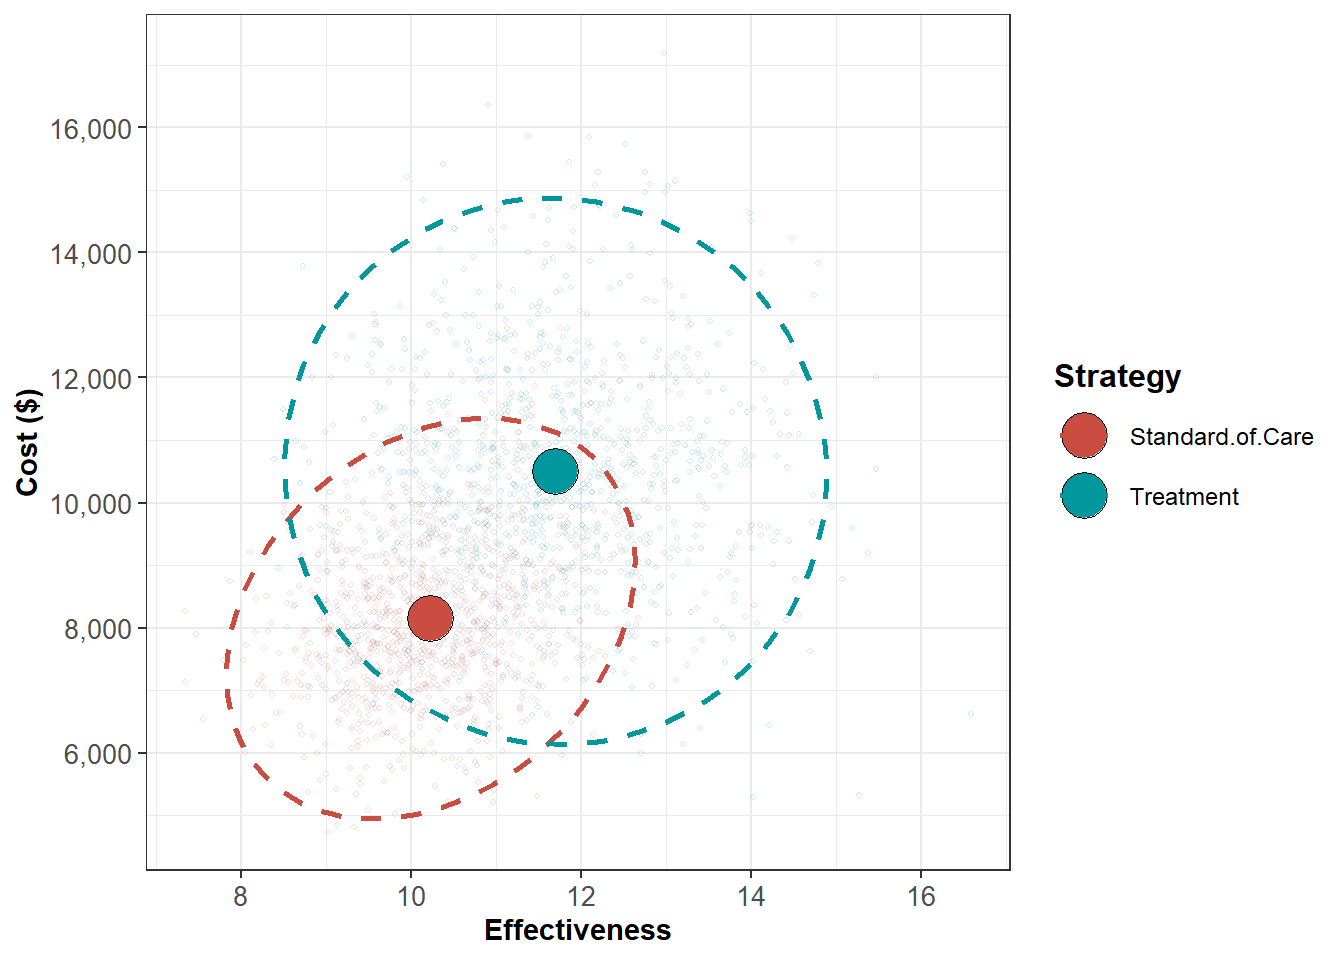
\includegraphics{Markov_3state_hesim_files/figure-latex/unnamed-chunk-28-1.pdf}

\hypertarget{conduct-cea-with-probabilistic-output}{%
\subsection{08.4.3 Conduct CEA with probabilistic
output}\label{conduct-cea-with-probabilistic-output}}

\begin{Shaded}
\begin{Highlighting}[]
\CommentTok{# Compute expected costs and effects for each strategy from the PSA}
\NormalTok{df_out_ce_psa <-}\StringTok{ }\KeywordTok{summary}\NormalTok{(l_psa)}

\CommentTok{# Calculate incremental cost-effectiveness ratios (ICERs)}
\NormalTok{df_cea_psa <-}\StringTok{ }\KeywordTok{calculate_icers}\NormalTok{(}\DataTypeTok{cost       =}\NormalTok{ df_out_ce_psa}\OperatorTok{$}\NormalTok{meanCost, }
                              \DataTypeTok{effect     =}\NormalTok{ df_out_ce_psa}\OperatorTok{$}\NormalTok{meanEffect,}
                              \DataTypeTok{strategies =}\NormalTok{ df_out_ce_psa}\OperatorTok{$}\NormalTok{Strategy)}
\NormalTok{df_cea_psa}
\end{Highlighting}
\end{Shaded}

\begin{verbatim}
##           Strategy      Cost   Effect Inc_Cost Inc_Effect     ICER Status
## 1 Standard.of.Care  8148.004 10.28706       NA         NA       NA     ND
## 2        Treatment 16149.044 11.74808  8001.04   1.461028 5476.307     ND
\end{verbatim}

\hypertarget{plot-cost-effectiveness-frontier}{%
\subsection{08.4.4 Plot cost-effectiveness
frontier}\label{plot-cost-effectiveness-frontier}}

\begin{Shaded}
\begin{Highlighting}[]
\KeywordTok{plot}\NormalTok{(df_cea_psa)}
\end{Highlighting}
\end{Shaded}

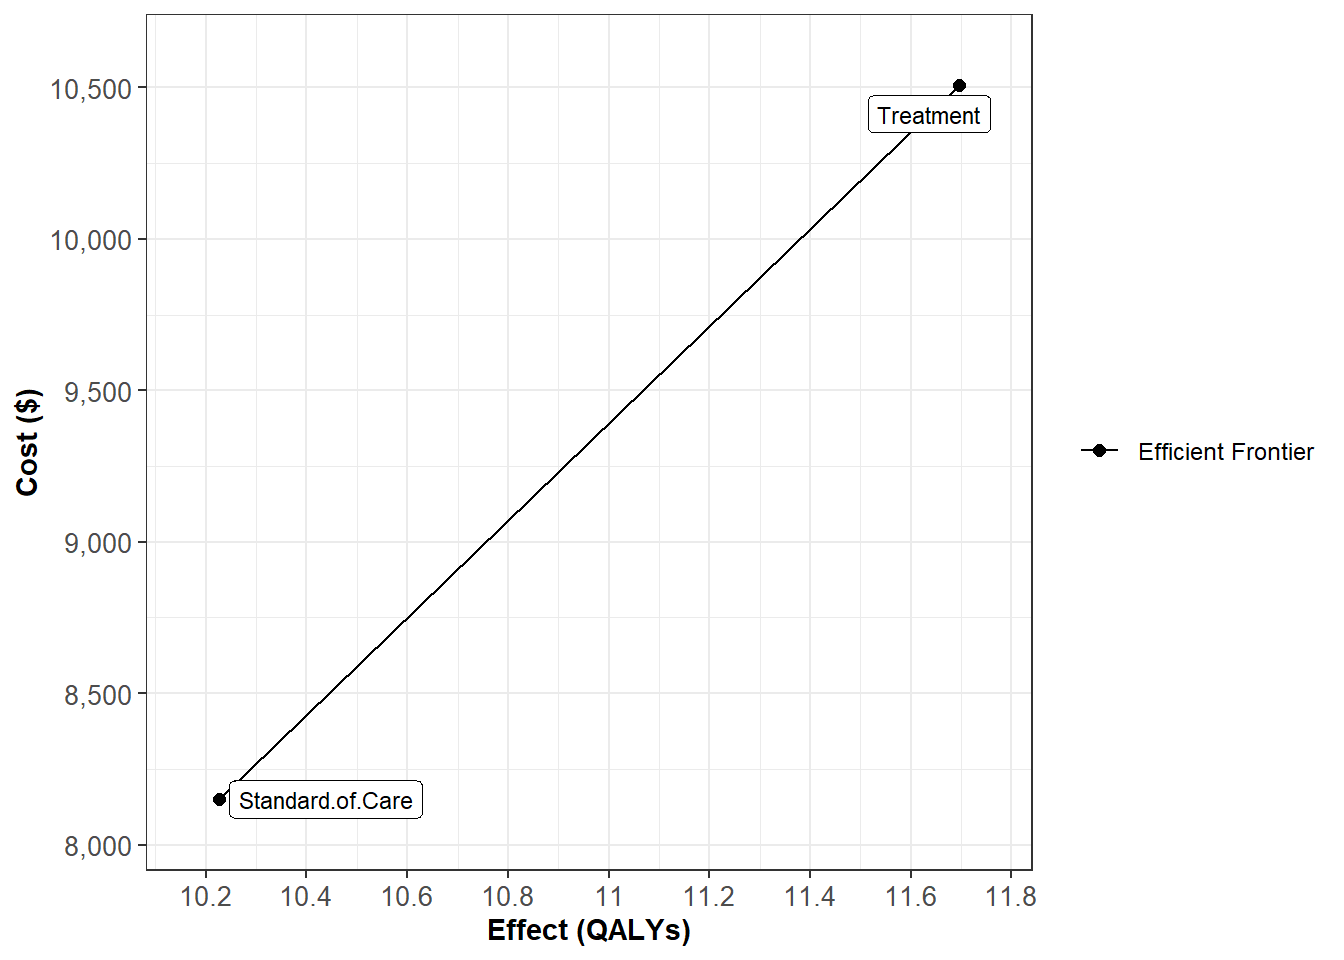
\includegraphics{Markov_3state_hesim_files/figure-latex/unnamed-chunk-30-1.pdf}

\hypertarget{cost-effectiveness-acceptability-curves-ceacs-and-frontier-ceaf}{%
\subsection{08.4.5 Cost-effectiveness acceptability curves (CEACs) and
frontier
(CEAF)}\label{cost-effectiveness-acceptability-curves-ceacs-and-frontier-ceaf}}

\begin{Shaded}
\begin{Highlighting}[]
\NormalTok{ceac_obj <-}\StringTok{ }\KeywordTok{ceac}\NormalTok{(}\DataTypeTok{wtp =}\NormalTok{ v_wtp, }\DataTypeTok{psa =}\NormalTok{ l_psa)}
\CommentTok{# Regions of highest probability of cost-effectiveness for each strategy}
\KeywordTok{summary}\NormalTok{(ceac_obj)}
\end{Highlighting}
\end{Shaded}

\begin{verbatim}
##   range_min range_max   cost_eff_strat
## 1         0      5000 Standard.of.Care
\end{verbatim}

\begin{Shaded}
\begin{Highlighting}[]
\CommentTok{# CEAC & CEAF plot}
\KeywordTok{plot}\NormalTok{(ceac_obj)}
\end{Highlighting}
\end{Shaded}

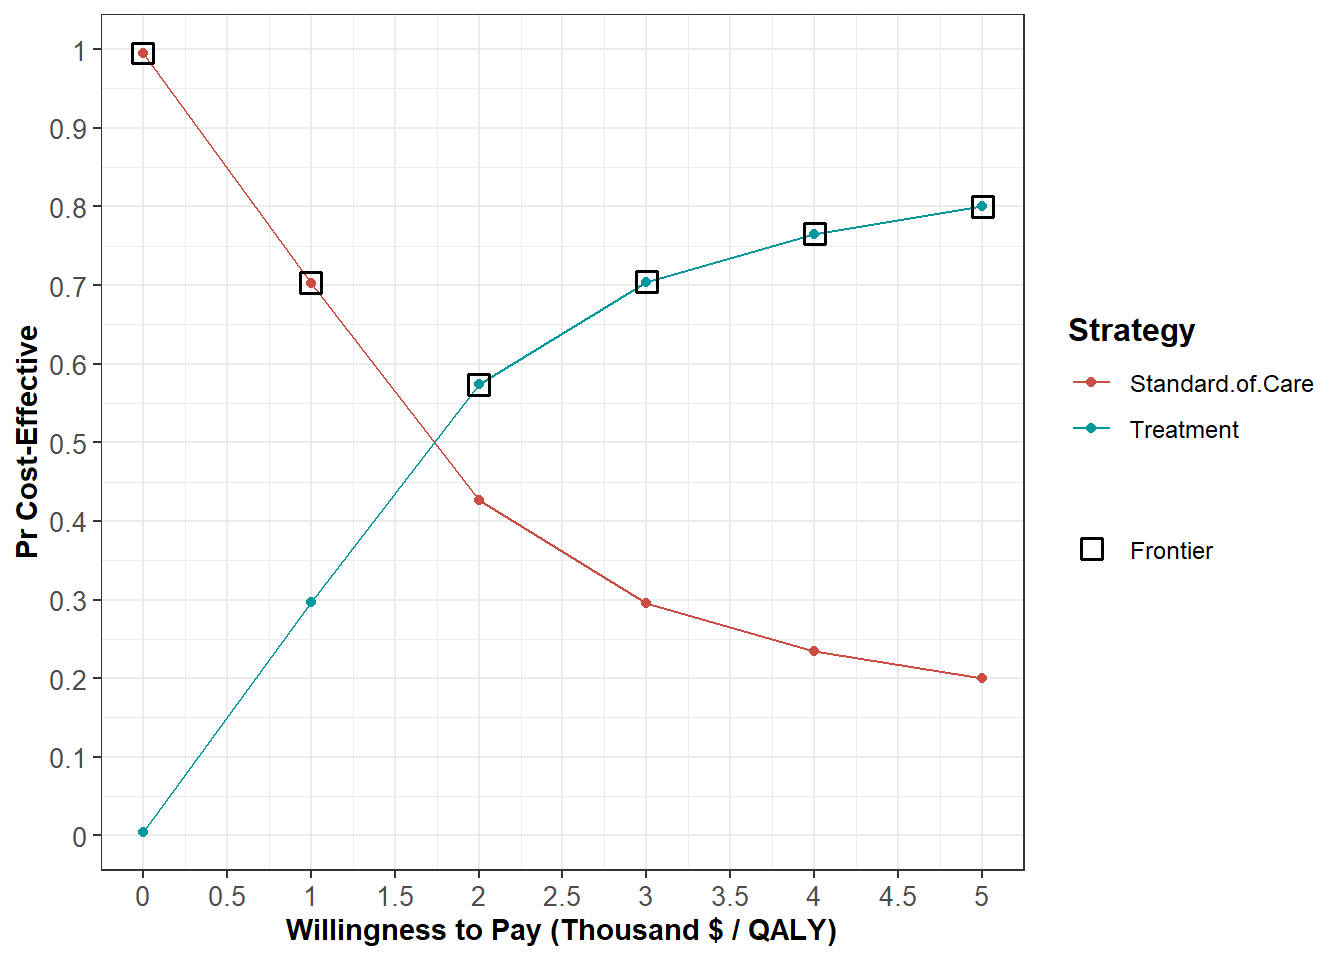
\includegraphics{Markov_3state_hesim_files/figure-latex/unnamed-chunk-31-1.pdf}

\hypertarget{expected-loss-curves-elcs}{%
\subsection{08.4.6 Expected Loss Curves
(ELCs)}\label{expected-loss-curves-elcs}}

The expected loss is the the quantification of the foregone benefits
when choosing a suboptimal strategy given current evidence.

\begin{Shaded}
\begin{Highlighting}[]
\NormalTok{elc_obj <-}\StringTok{ }\KeywordTok{calc_exp_loss}\NormalTok{(}\DataTypeTok{wtp =}\NormalTok{ v_wtp, }\DataTypeTok{psa =}\NormalTok{ l_psa)}
\NormalTok{elc_obj}
\end{Highlighting}
\end{Shaded}

\begin{verbatim}
##     WTP         Strategy Expected_Loss On_Frontier
## 1     0 Standard.of.Care       0.00000        TRUE
## 2     0        Treatment    8001.03979       FALSE
## 3  1000 Standard.of.Care       0.00000        TRUE
## 4  1000        Treatment    6540.01147       FALSE
## 5  2000 Standard.of.Care      38.76766        TRUE
## 6  2000        Treatment    5117.75081       FALSE
## 7  3000 Standard.of.Care     322.26595        TRUE
## 8  3000        Treatment    3940.22079       FALSE
## 9  4000 Standard.of.Care     989.52884        TRUE
## 10 4000        Treatment    3146.45536       FALSE
## 11 5000 Standard.of.Care    1937.60524        TRUE
## 12 5000        Treatment    2633.50344       FALSE
\end{verbatim}

\begin{Shaded}
\begin{Highlighting}[]
\CommentTok{# ELC plot}
\KeywordTok{plot}\NormalTok{(elc_obj, }\DataTypeTok{log_y =} \OtherTok{FALSE}\NormalTok{)}
\end{Highlighting}
\end{Shaded}

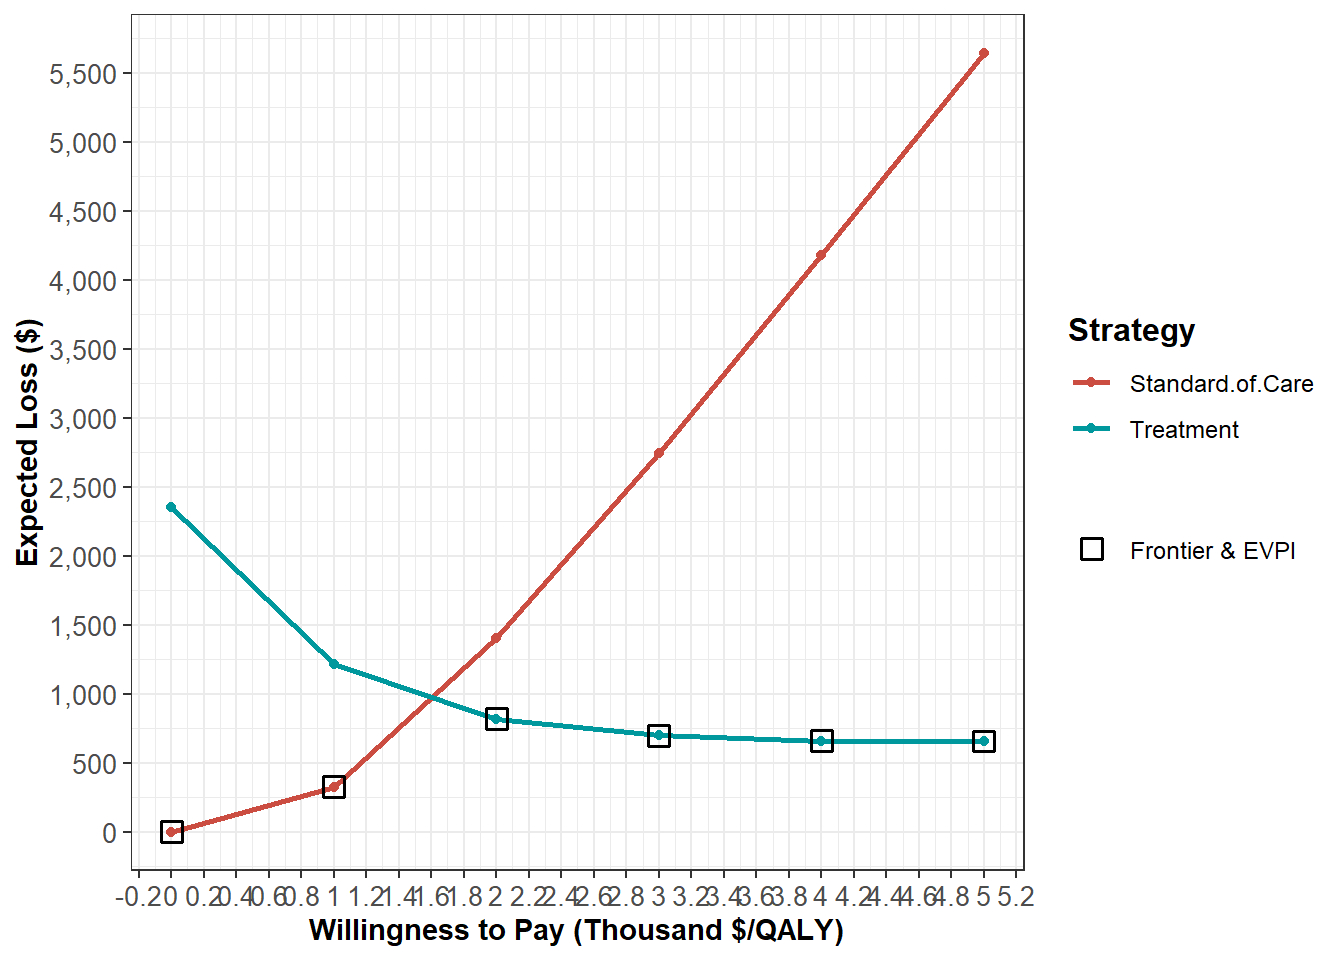
\includegraphics{Markov_3state_hesim_files/figure-latex/unnamed-chunk-32-1.pdf}

\hypertarget{expected-value-of-perfect-information-evpi}{%
\subsection{08.4.7 Expected value of perfect information
(EVPI)}\label{expected-value-of-perfect-information-evpi}}

\begin{Shaded}
\begin{Highlighting}[]
\NormalTok{evpi <-}\StringTok{ }\KeywordTok{calc_evpi}\NormalTok{(}\DataTypeTok{wtp =}\NormalTok{ v_wtp, }\DataTypeTok{psa =}\NormalTok{ l_psa)}
\CommentTok{# EVPI plot}
\KeywordTok{plot}\NormalTok{(evpi, }\DataTypeTok{effect_units =} \StringTok{"QALY"}\NormalTok{)}
\end{Highlighting}
\end{Shaded}

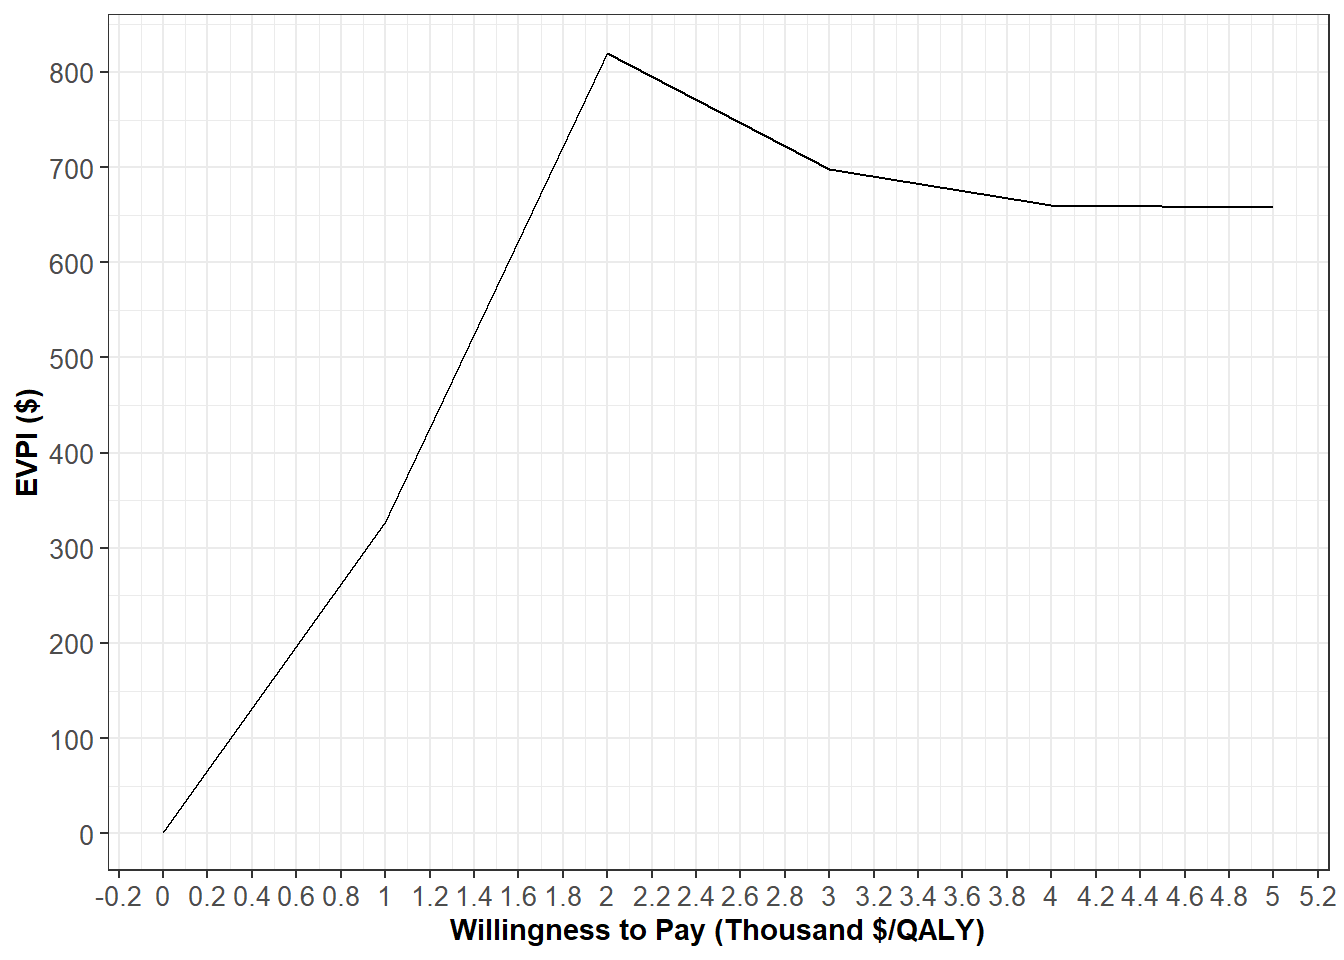
\includegraphics{Markov_3state_hesim_files/figure-latex/unnamed-chunk-33-1.pdf}

\hypertarget{using-r-package-hesim}{%
\section{\texorpdfstring{09 Using \texttt{R} package
\texttt{hesim}}{09 Using R package hesim}}\label{using-r-package-hesim}}

\begin{Shaded}
\begin{Highlighting}[]
\KeywordTok{p_load}\NormalTok{(}\StringTok{"hesim"}\NormalTok{)}
\end{Highlighting}
\end{Shaded}

\hypertarget{model-setup}{%
\subsection{09.1 Model setup}\label{model-setup}}

Here we define target population and intervention strategies.

We have one representative patient here of age 25, we can think of this
as a cohort of homogenous patients instead of one individual patient.

\begin{Shaded}
\begin{Highlighting}[]
\CommentTok{# define strategies}
\NormalTok{strategies <-}\StringTok{ }\KeywordTok{data.frame}\NormalTok{(}
  \DataTypeTok{strategy_id   =} \DecValTok{1}\OperatorTok{:}\NormalTok{n_str,}
  \DataTypeTok{strategy_name =}\NormalTok{ v_names_str}
\NormalTok{  )}
\CommentTok{# define patient cohort}
\NormalTok{patients <-}\StringTok{ }\KeywordTok{data.frame}\NormalTok{(}
  \DataTypeTok{patient_id =} \DecValTok{1}\NormalTok{,}
  \DataTypeTok{age        =} \DecValTok{25}
\NormalTok{)}
\CommentTok{# create dataset with }
\NormalTok{hesim_dat <-}\StringTok{ }\KeywordTok{hesim_data}\NormalTok{(}
  \DataTypeTok{strategies =}\NormalTok{ strategies,}
  \DataTypeTok{patients   =}\NormalTok{ patients}
\NormalTok{)}
\NormalTok{hesim_dat}
\end{Highlighting}
\end{Shaded}

\begin{verbatim}
## $strategies
##   strategy_id    strategy_name
## 1           1 Standard of Care
## 2           2        Treatment
## 
## $patients
##   patient_id age
## 1          1  25
## 
## attr(,"class")
## [1] "hesim_data"
\end{verbatim}

\hypertarget{parameters}{%
\subsection{09.2 parameters}\label{parameters}}

\begin{Shaded}
\begin{Highlighting}[]
\NormalTok{params <-}\StringTok{ }\KeywordTok{list}\NormalTok{(}
  \CommentTok{# medical costs}
  \DataTypeTok{c_medical    =} \KeywordTok{c}\NormalTok{(}\DataTypeTok{Healthy =}\NormalTok{ c_H, }\DataTypeTok{Sick =}\NormalTok{ c_S),}
  \DataTypeTok{c_medical_se =} \KeywordTok{c}\NormalTok{(}\DataTypeTok{Healthy =} \DecValTok{100}\NormalTok{, }\DataTypeTok{Sick =} \DecValTok{100}\NormalTok{),}
  \CommentTok{# treatment costs (embedded in medical costs since only those who are sick get treated)}
  \DataTypeTok{c_trt  =}\NormalTok{ c_trt,}
  \CommentTok{# state utilities}
  \DataTypeTok{u_mean =} \KeywordTok{c}\NormalTok{(}\DataTypeTok{Healthy =}\NormalTok{ u_H,  }\DataTypeTok{Sick =}\NormalTok{ u_S),}
  \DataTypeTok{u_se   =} \KeywordTok{c}\NormalTok{(}\DataTypeTok{Healthy =} \FloatTok{0.05}\NormalTok{, }\DataTypeTok{Sick =} \FloatTok{0.05}\NormalTok{)}
\NormalTok{)}
\end{Highlighting}
\end{Shaded}

\hypertarget{psa-setup}{%
\subsection{09.3 PSA setup}\label{psa-setup}}

\texttt{rng\_def()}

\begin{Shaded}
\begin{Highlighting}[]
\NormalTok{rng_def <-}\StringTok{ }\KeywordTok{define_rng}\NormalTok{(\{}
  \KeywordTok{list}\NormalTok{( }\CommentTok{# Parameters to return}
    \CommentTok{# medical costs}
    \DataTypeTok{c_medical =} \KeywordTok{gamma_rng}\NormalTok{(}\DataTypeTok{mean =}\NormalTok{ c_medical, }\DataTypeTok{sd =}\NormalTok{ c_medical_se),}
    \DataTypeTok{c_trt     =} \KeywordTok{gamma_rng}\NormalTok{(}\DataTypeTok{mean =}\NormalTok{ c_trt,     }\DataTypeTok{sd =} \DecValTok{1000}\NormalTok{),}
    \CommentTok{# state utilities}
    \DataTypeTok{u =} \KeywordTok{beta_rng}\NormalTok{(}\DataTypeTok{mean =}\NormalTok{ u_mean, }\DataTypeTok{sd =}\NormalTok{ u_se)}
\NormalTok{  )}
\NormalTok{\}, }\DataTypeTok{n =} \DecValTok{1000}\NormalTok{)}
\end{Highlighting}
\end{Shaded}

\hypertarget{transform-parameters}{%
\subsection{09.4 Transform parameters}\label{transform-parameters}}

\begin{Shaded}
\begin{Highlighting}[]
\NormalTok{input_data <-}\StringTok{ }\NormalTok{hesim}\OperatorTok{::}\KeywordTok{expand}\NormalTok{(hesim_dat, }\DataTypeTok{by =} \KeywordTok{c}\NormalTok{(}\StringTok{"strategies"}\NormalTok{, }\StringTok{"patients"}\NormalTok{))}
\KeywordTok{head}\NormalTok{(input_data)}
\end{Highlighting}
\end{Shaded}

\begin{verbatim}
##    strategy_id patient_id    strategy_name age
## 1:           1          1 Standard of Care  25
## 2:           2          1        Treatment  25
\end{verbatim}

The function \texttt{define\_tparams()} returns:

\begin{itemize}
\item
  \texttt{tpmatrix}: The transition probability matrix
\item
  \texttt{utility}: Utility assigned to each health state
\item
  \texttt{costs}: Costs assigned to each health state or each cost
  category
\end{itemize}

Your task: write mathematical expressions

The function: automatically loops over PSA iterations (running the model
on each sampled parameter set)

\begin{Shaded}
\begin{Highlighting}[]
\NormalTok{tparams_def <-}\StringTok{ }\KeywordTok{define_tparams}\NormalTok{(\{}
  \CommentTok{# treatment reduces the risk of getting sick}
\NormalTok{  rr <-}\StringTok{ }\KeywordTok{ifelse}\NormalTok{(strategy_name }\OperatorTok{==}\StringTok{ "Standard of Care"}\NormalTok{, }\DecValTok{1}\NormalTok{, p_HS_trt }\OperatorTok{/}\StringTok{ }\NormalTok{p_HS) }\CommentTok{# relative risk}
  
  \KeywordTok{list}\NormalTok{(}
    \DataTypeTok{tpmatrix =} \KeywordTok{tpmatrix}\NormalTok{(}
\NormalTok{      (}\DecValTok{1} \OperatorTok{-}\StringTok{ }\NormalTok{p_HD) }\OperatorTok{*}\StringTok{ }\NormalTok{(}\DecValTok{1} \OperatorTok{-}\StringTok{ }\NormalTok{p_HS }\OperatorTok{*}\StringTok{ }\NormalTok{rr),  (}\DecValTok{1} \OperatorTok{-}\StringTok{ }\NormalTok{p_HD) }\OperatorTok{*}\StringTok{ }\NormalTok{(p_HS }\OperatorTok{*}\StringTok{ }\NormalTok{rr),  p_HD,  }
       \DecValTok{0}\NormalTok{,  C,  p_SD,}
       \DecValTok{0}\NormalTok{,  }\DecValTok{0}\NormalTok{,  }\DecValTok{1}          
\NormalTok{    ),}
    
    \DataTypeTok{utility =}\NormalTok{ u,}
    \DataTypeTok{costs =} \KeywordTok{list}\NormalTok{(}
      \DataTypeTok{treatment =} \KeywordTok{ifelse}\NormalTok{(strategy_name }\OperatorTok{==}\StringTok{ "Standard of Care"}\NormalTok{, }\DecValTok{0}\NormalTok{, c_trt),}
      \DataTypeTok{medical   =}\NormalTok{ c_medical}
\NormalTok{    )}
\NormalTok{  )}
\NormalTok{\})}
\end{Highlighting}
\end{Shaded}

\hypertarget{simulation}{%
\subsection{09.5 Simulation}\label{simulation}}

Construct model:

\begin{Shaded}
\begin{Highlighting}[]
\NormalTok{mod_def <-}\StringTok{ }\KeywordTok{define_model}\NormalTok{(}\DataTypeTok{tparams_def =}\NormalTok{ tparams_def, }
                        \DataTypeTok{rng_def     =}\NormalTok{ rng_def, }
                        \DataTypeTok{params      =}\NormalTok{ params)}
\end{Highlighting}
\end{Shaded}

Initialize-model:

\begin{Shaded}
\begin{Highlighting}[]
\NormalTok{cost_args <-}\StringTok{ }\KeywordTok{list}\NormalTok{(}
  \DataTypeTok{treatment =} \KeywordTok{list}\NormalTok{(}\DataTypeTok{method =} \StringTok{"starting"}\NormalTok{),}
  \DataTypeTok{medical   =} \KeywordTok{list}\NormalTok{(}\DataTypeTok{method =} \StringTok{"wlos"}\NormalTok{)}
\NormalTok{)}
\NormalTok{econmod <-}\StringTok{ }\KeywordTok{create_CohortDtstm}\NormalTok{(mod_def, input_data, }\DataTypeTok{cost_args =}\NormalTok{ cost_args)}
\end{Highlighting}
\end{Shaded}

Simulate outcomes:

\begin{Shaded}
\begin{Highlighting}[]
\NormalTok{econmod}\OperatorTok{$}\KeywordTok{sim_stateprobs}\NormalTok{(}\DataTypeTok{n_cycles =}\NormalTok{ n_t)}
\KeywordTok{head}\NormalTok{(econmod}\OperatorTok{$}\NormalTok{stateprobs_)}
\end{Highlighting}
\end{Shaded}

\begin{verbatim}
##    sample strategy_id patient_id grp_id state_id t      prob
## 1:      1           1          1      1        1 0 1.0000000
## 2:      1           1          1      1        1 1 0.9310000
## 3:      1           1          1      1        1 2 0.8667610
## 4:      1           1          1      1        1 3 0.8069545
## 5:      1           1          1      1        1 4 0.7512746
## 6:      1           1          1      1        1 5 0.6994367
\end{verbatim}

\begin{Shaded}
\begin{Highlighting}[]
\NormalTok{econmod}\OperatorTok{$}\KeywordTok{sim_qalys}\NormalTok{(}\DataTypeTok{dr =}\NormalTok{ d_e, }\DataTypeTok{lys =} \OtherTok{TRUE}\NormalTok{, }\DataTypeTok{integrate_method =} \StringTok{"riemann_right"}\NormalTok{)}
\KeywordTok{head}\NormalTok{(econmod}\OperatorTok{$}\NormalTok{qalys_)}
\end{Highlighting}
\end{Shaded}

\begin{verbatim}
##    sample strategy_id patient_id grp_id state_id   dr    qalys       lys
## 1:      1           1          1      1        1 0.03 6.484607  9.339850
## 2:      1           1          1      1        2 0.03 1.841271  3.861427
## 3:      1           2          1      1        1 0.03 8.199613 11.809992
## 4:      1           2          1      1        2 0.03 1.361197  2.854639
## 5:      2           1          1      1        1 0.03 8.063655  9.339850
## 6:      2           1          1      1        2 0.03 1.849052  3.861427
\end{verbatim}

\begin{Shaded}
\begin{Highlighting}[]
\NormalTok{econmod}\OperatorTok{$}\KeywordTok{sim_costs}\NormalTok{(}\DataTypeTok{dr =}\NormalTok{ d_c, }\DataTypeTok{integrate_method =} \StringTok{"riemann_right"}\NormalTok{)}
\KeywordTok{head}\NormalTok{(econmod}\OperatorTok{$}\NormalTok{costs_)}
\end{Highlighting}
\end{Shaded}

\begin{verbatim}
##    sample strategy_id patient_id grp_id state_id   dr  category    costs
## 1:      1           1          1      1        1 0.03 treatment    0.000
## 2:      1           1          1      1        2 0.03 treatment    0.000
## 3:      1           2          1      1        1 0.03 treatment 7819.843
## 4:      1           2          1      1        2 0.03 treatment    0.000
## 5:      2           1          1      1        1 0.03 treatment    0.000
## 6:      2           1          1      1        2 0.03 treatment    0.000
\end{verbatim}

\hypertarget{cost-effectivess-analysis}{%
\subsection{09.6 Cost-effectivess
analysis}\label{cost-effectivess-analysis}}

\begin{Shaded}
\begin{Highlighting}[]
\NormalTok{ce_sim <-}\StringTok{ }\NormalTok{econmod}\OperatorTok{$}\KeywordTok{summarize}\NormalTok{()}
\NormalTok{cea_pw_out <-}\StringTok{ }\KeywordTok{cea_pw}\NormalTok{(ce_sim, }
                     \DataTypeTok{comparator =} \DecValTok{1}\NormalTok{, }
                     \DataTypeTok{dr_qalys =} \FloatTok{0.03}\NormalTok{, }\DataTypeTok{dr_costs =} \FloatTok{0.03}\NormalTok{,}
                     \DataTypeTok{k =} \KeywordTok{seq}\NormalTok{(}\DecValTok{0}\NormalTok{, }\DecValTok{5000}\NormalTok{, }\DecValTok{1000}\NormalTok{))}

\CommentTok{## @knitr icer}
\KeywordTok{icer_tbl}\NormalTok{(cea_pw_out, }\DataTypeTok{colnames =}\NormalTok{ strategies}\OperatorTok{$}\NormalTok{strategy_name) }
\end{Highlighting}
\end{Shaded}

\begin{verbatim}
##                   Standard of Care Treatment                
## Incremental QALYs "-"              "1.47 (1.21, 1.72)"      
## Incremental costs "-"              "7,990 (6,070, 10,233)"  
## Incremental NMB   "-"              "65,685 (52,214, 77,821)"
## ICER              "-"              "5,422"                  
## Conclusion        "-"              "Cost-effective"
\end{verbatim}

\hypertarget{overview-of-hesim}{%
\section{\texorpdfstring{10 Overview of
\texttt{hesim}}{10 Overview of hesim}}\label{overview-of-hesim}}

\textbf{Advantages}:

\begin{itemize}
\item
  Easy to build models without having to program the complete model
  structure (easier for novice modelers).
\item
  A lot of the modeling code are implemented for you in the back end.
\item
  Suitable for modelers who are not familiar with \texttt{R} programming
  and functionality.
\item
  Code written in \texttt{C++} in the back end, which offers enhanced
  computational speed.
\end{itemize}

\textbf{Disadvantages}:

\begin{itemize}
\item
  Its rigid function structure inhibits its ability tweak models or
  incorporate more complex model components (e.g.~tunnel states,
  transition rewards).
\item
  Does not provide the option for running deterministic analysis or
  one-way and two-way sensitivity analyses.
\item
  Does not provide the ability to capture information about the specific
  transitions among health states (transition dynamics).
\item
  Does not provide the ability to easily compute epidemiological
  outcomes.
\item
  Does not allow costs to be applied to certain health states (at least
  not easily).
\end{itemize}

\hypertarget{references}{%
\section{References}\label{references}}

\begin{Shaded}
\begin{Highlighting}[]
\KeywordTok{citation}\NormalTok{(}\StringTok{"hesim"}\NormalTok{)}
\end{Highlighting}
\end{Shaded}

\begin{verbatim}
## 
## To cite package 'hesim' in publications use:
## 
##   Devin Incerti and Jeroen P. Jansen (2020). hesim: Health-Economic
##   Simulation Modeling and Decision Analysis. R package version 0.4.1.
##   https://CRAN.R-project.org/package=hesim
## 
## A BibTeX entry for LaTeX users is
## 
##   @Manual{,
##     title = {hesim: Health-Economic Simulation Modeling and Decision Analysis},
##     author = {Devin Incerti and Jeroen P. Jansen},
##     year = {2020},
##     note = {R package version 0.4.1},
##     url = {https://CRAN.R-project.org/package=hesim},
##   }
\end{verbatim}

\end{document}
